        %%******************************************%%
        %%                                          %%
        %%        Modello di tesi di laurea         %%
        %%            di Andrea Giraldin            %%
        %%                                          %%
        %%             2 novembre 2012              %%
        %%                                          %%
        %%******************************************%%


% I seguenti commenti speciali impostano:
% 1. 
% 2. PDFLaTeX come motore di composizione;
% 3. tesi.tex come documento principale;
% 4. il controllo ortografico italiano per l'editor.

% !TEX encoding = UTF-8
% !TEX TS-program = pdflatex
% !TEX root = tesi.tex
% !TEX spellcheck = it-IT

\documentclass[10pt,                    % corpo del font principale
               a4paper,                 % carta A4
               twoside,                 % impagina per fronte-retro
               openright,               % inizio capitoli a destra
               english,                 
               italian,                 
               ]{book}    

%**************************************************************
% Importazione package
%************************************************************** 

%\usepackage{amsmath,amssymb,amsthm}    % matematica

\usepackage[T1]{fontenc}                % codifica dei font:
                                        % NOTA BENE! richiede una distribuzione *completa* di LaTeX

\usepackage[utf8]{inputenc}             % codifica di input; anche [latin1] va bene
                                        % NOTA BENE! va accordata con le preferenze dell'editor

\usepackage[english, italian]{babel}    % per scrivere in italiano e in inglese;
                                        % l'ultima lingua (l'italiano) risulta predefinita

\usepackage{bookmark}                   % segnalibri

\usepackage{caption}                    % didascalie

\usepackage{chngpage,calc}              % centra il frontespizio

\usepackage{csquotes}                   % gestisce automaticamente i caratteri (")

\usepackage{emptypage}                  % pagine vuote senza testatina e piede di pagina

\usepackage{epigraph}					% per epigrafi

\usepackage{eurosym}                    % simbolo dell'euro

%\usepackage{indentfirst}               % rientra il primo paragrafo di ogni sezione

\usepackage{graphicx}                   % immagini

\usepackage{hyperref}                   % collegamenti ipertestuali

\usepackage[binding=5mm]{layaureo}      % margini ottimizzati per l'A4; rilegatura di 5 mm

\usepackage{listings}                   % codici

\usepackage{microtype}                  % microtipografia

\usepackage{mparhack,fixltx2e,relsize}  % finezze tipografiche

\usepackage{nameref}                    % visualizza nome dei riferimenti                                      

\usepackage[font=small]{quoting}        % citazioni

\usepackage{subfig}                     % sottofigure, sottotabelle

\usepackage[italian]{varioref}          % riferimenti completi della pagina

\usepackage[dvipsnames]{xcolor}         % colori

\usepackage{booktabs}                   % tabelle                                       
\usepackage{tabularx}                   % tabelle di larghezza prefissata                                    
\usepackage{longtable}                  % tabelle su più pagine                                        
\usepackage{ltxtable}                   % tabelle su più pagine e adattabili in larghezza

\usepackage[T1]{fontenc}
\usepackage{lmodern}

\usepackage[toc, acronym]{glossaries}   % glossario
                                        % per includerlo nel documento bisogna:
                                        % 1. compilare una prima volta tesi.tex;
                                        % 2. eseguire: makeindex -s tesi.ist -t tesi.glg -o tesi.gls tesi.glo
                                        % 3. eseguire: makeindex -s tesi.ist -t tesi.alg -o tesi.acr tesi.acn
                                        % 4. compilare due volte tesi.tex.

\usepackage[backend=biber,style=verbose-ibid,hyperref,backref]{biblatex}
                                        % eccellente pacchetto per la bibliografia; 
                                        % produce uno stile di citazione autore-anno; 
                                        % lo stile "numeric-comp" produce riferimenti numerici
                                        % per includerlo nel documento bisogna:
                                        % 1. compilare una prima volta tesi.tex;
                                        % 2. eseguire: biber tesi
                                        % 3. compilare ancora tesi.tex.

%**************************************************************
% file contenente le impostazioni della tesi
%**************************************************************

%**************************************************************
% Frontespizio
%**************************************************************

% Autore
\newcommand{\myName}{Massimo Toffoletto}                                    
\newcommand{\myTitle}{Riconoscimento del linguaggio naturale per assistenti virtuali: interpretazione e apprendimento di comandi vocali}

% Tipo di tesi                   
\newcommand{\myDegree}{Tesi di laurea triennale}

% Università             
\newcommand{\myUni}{Università degli Studi di Padova}

% Facoltà       
\newcommand{\myFaculty}{Corso di Laurea in Informatica}

% Dipartimento
\newcommand{\myDepartment}{Dipartimento di Matematica "Tullio Levi-Civita"}

% Titolo del relatore
\newcommand{\profTitle}{Prof.}

% Relatore
\newcommand{\myProf}{Paolo Baldan}

% Luogo
\newcommand{\myLocation}{Padova}

% Anno accademico
\newcommand{\myAA}{2019-2020}

% Data discussione
\newcommand{\myTime}{Luglio 2020}


%**************************************************************
% Impostazioni di impaginazione
% see: http://wwwcdf.pd.infn.it/AppuntiLinux/a2547.htm
%**************************************************************

\setlength{\parindent}{14pt}   % larghezza rientro della prima riga
\setlength{\parskip}{0pt}   % distanza tra i paragrafi


%**************************************************************
% Impostazioni di biblatex
%**************************************************************
\bibliography{bibliografia} % database di biblatex 

\defbibheading{bibliography} {
    \cleardoublepage
    \phantomsection 
    \addcontentsline{toc}{chapter}{\bibname}
    \chapter*{\bibname\markboth{\bibname}{\bibname}}
}

\setlength\bibitemsep{1.5\itemsep} % spazio tra entry

\DeclareBibliographyCategory{opere}
\DeclareBibliographyCategory{web}

\addtocategory{opere}{womak:lean-thinking}
\addtocategory{web}{site:agile-manifesto}

\defbibheading{opere}{\section*{Riferimenti bibliografici}}
\defbibheading{web}{\section*{Siti Web consultati}}


%**************************************************************
% Impostazioni di caption
%**************************************************************
\captionsetup{
    tableposition=top,
    figureposition=bottom,
    font=small,
    format=hang,
    labelfont=bf
}

%**************************************************************
% Impostazioni di glossaries
%**************************************************************

%**************************************************************
% Acronimi
%**************************************************************
\renewcommand{\acronymname}{Acronimi e abbreviazioni}

\newacronym[description={\glslink{apig}{Application Program Interface}}]
{api}{API}{Application Program Interface}

\newacronym[description={\glslink{erpg}{Enterprise Resource Planning}}]
{erp}{ERP}{Enterprise Resource Planning}

\newacronym[description={\glslink{ibmg}{International Business Machines Corporation}}]
{ibm}{IBM}{International Business Machines Corporation}

\newacronym[description={\glslink{nlug}{Natural Language Understanding}}]
{nlu}{NLU}{Natural Language Understanding}

\newacronym[description={\glslink{pocg}{Proof of Concept}}]
{poc}{PoC}{Proof of Concept}

\newacronym[description={\glslink{jvmg}{Java Virtual Machine}}]
{jvm}{JVM}{Java Virtual Machine}

\newacronym[description={\glslink{es6}{ECMAScript6}}]
{es6}{ES6}{ECMAScript6}

\newacronym[description={\glslink{html}{HyperText Markup Language}}]
{html}{HTML}{HyperText Markup Language}

\newacronym[description={\glslink{css}{Cascading Style Sheets}}]
{css}{CSS}{Cascading Style Sheets}

\newacronym[description={\glslink{php}{Hypertext Preprocessor}}]
{php}{PHP}{Hypertext Preprocessor}

\newacronym[description={\glslink{ram}{Random Access Memory}}]
{ram}{RAM}{Random Access Memory}

\newacronym[description={\glslink{sdk}{Software Development Kit}}]
{sdk}{SDK}{Software Development Kit}

\newacronym[description={\glslink{http}{HyperText Transfer Protocol}}]
{http}{HTTP}{HyperText Transfer Protocol}
%**************************************************************
% Glossario
%**************************************************************
\renewcommand{\glossaryname}{Glossario}

\newglossaryentry{apig}
{
	name=\glslink{api}{API},
	text=Application Program Interface,
	sort=api,
	description={in informatica con il termine \emph{Application Programming Interface API} (ing. interfaccia di programmazione di un'applicazione) si indica ogni insieme di procedure disponibili al programmatore, di solito raggruppate a formare un set di strumenti specifici per l'espletamento di un determinato compito all'interno di un certo programma. La finalità è ottenere un'astrazione, di solito tra l'hardware e il programmatore o tra software a basso e quello ad alto livello semplificando così il lavoro di programmazione}
}


\newglossaryentry{erpg}
{
    name=\glslink{erp}{ERP},
    text=ERP,
    sort=erp,
    description={in informatica con il termine \emph{ERP, Enterprise Resource Planning} (ing. pianificazione delle risorse d'impresa) è un software di gestione che integra tutti i processi di business rilevanti di un'azienda e tutte le sue funzioni quali vendite, acquisti, gestione magazzino, finanza e contabilità. Integra quindi tutte le attività aziendali in un unico sistema che risulta essere indispensabile per supportare il Management.}
}

\newglossaryentry{ibmg}
{
	name=\glslink{ibm}{IBM},
	text=IBM,
	sort=ibm,
	description={L'\emph{IBM, International Business Machines Corporation} è un'azienda statunitense, la più antica e tra le maggiori al mondo nel settore informatico. Produce e commercializza hardware, software per computer, middleware e servizi informatici, offrendo anche infrastrutture, servizi di hosting, cloud computing, intelligenza artificiale e consulenza nel settore informatico e strategico.}
}

\newglossaryentry{nlug}
{
	name=\glslink{nlu}{NLU},
	text=NLU,
	sort=ibm,
	description={La \emph{NLU, Natural Language Understanding} (ing. comprensione del linguaggio naturale) è un ramo dell'elaborazione del linguaggio naturale nell'intelligenza artificiale.}
}

\newglossaryentry{pocg}
{
	name=\glslink{pocg}{PoC},
	text=PoC,
	sort=poc,
	description={Con \emph{PoC, Proof of Concept} (ing. prova di fattibilità) si intende una realizzazione incompleta o abbozzata di un determinato progetto o metodo, allo scopo di provarne la fattibilità o dimostrare la fondatezza di alcuni principi o concetti costituenti. Un esempio tipico è quello di un prototipo.}
}

\newglossaryentry{jvmg}
{
	name=\glslink{jvmg}{JVM},
	text=JVM,
	sort=jvm,
	description={La \emph{JVM, Java Virtual Machine} è il componente della piattaforma Java che esegue i programmi tradotti in bytecode dopo una prima fase di compilazione. Alcuni dei linguaggi di programmazione che possono essere tradotti in bytecode sono Java, Kotlin e Scala.}
}

\newglossaryentry{ttg}
{
	name=\glslink{ttg}{Test di Turing},
	text=Test di Turing,
	sort=Test di Turing,
	description={Il \emph{Test di Turing} è un criterio costruito dallo scienziato Alan Turing nel 1950 per determinare se una macchina sia in grado di comprendere il linguaggio naturale e più in generale di pensare.}
}

\newglossaryentry{sdkg}
{
	name=\glslink{sdkg}{Software Development Kit},
	text=Software Development Kit,
	sort=Software Development Kit,
	description={Un \emph{SDK, Software Development Kit} (ing. pacchetto di sviluppo software) in informatica, indica un insieme di strumenti per lo sviluppo e la documentazione di software.}
}

\newglossaryentry{httpg}
{
	name=\glslink{httpg}{HyperText Transfer Protocol},
	text=HyperText Transfer Protocol,
	sort=HyperText Transfer Protocol,
	description={In informatica \emph{HTTP, HyperText Transfer Protocol} (ing. protocollo di trasferimento di un ipertesto) è un protocollo a livello applicativo usato come principale sistema per la trasmissione d'informazioni sul Web. Esiste una versione detta \emph{HTTPS, HyperText Transfer Protocol over Secure Socket Layer} che implementa le stesse funzionalità applicando uno strato di crittografia.}
}

\newglossaryentry{buildg}
{
	name=\glslink{buildg}{build},
	text=build,
	sort=build,
	description={Nello sviluppo del software, \emph{build} indica il processo di trasformazione del codice sorgente in un artefatto eseguibile.}
}

\newglossaryentry{firebaseg}
{
	name=\glslink{firebaseg}{Firebase},
	text=Firebase,
	sort=Firebase,
	description={\emph{Firebase} è una piattaforma di sviluppo per applicazioni Web e mobile sviluppata da Firebase Inc. nel 2011 e acquisita da Google nel 2014}
}

\newglossaryentry{authg}
{
	name=\glslink{firebaseg}{OAuth 2.0},
	text=OAuth 2.0,
	sort=OAuth 2.0,
	description={\emph{OAuth 2.0} è un protocollo di rete aperto e standard, progettato specificamente per lavorare con il protocollo \emph{HTTP}. Consente l'emissione di un token d'accesso da parte di un server che fornisce autorizzatizioni ad un client previa approvazione dell'utente proprietario della risorsa cui si intende accedere. Rispetto alla sua versione precedente presenta una chiara divisione dei ruoli, implementando un mediatore tra client e server.}
}

\newglossaryentry{rldg}
{
	name=\glslink{rldg}{Firebase},
	text=railroad,
	sort=railroad,
	description={I \emph{diagrammi railroad}, detti anche \emph{diagrammi di sintassi} consistono in una rapprensentazione grafica per grammatiche libere da contesto.}
}

\newglossaryentry{parsg}
{
	name=\glslink{parsg}{parser},
	text=parser,
	sort=parser,
	description={In informatica il \emph{parser} è un software che realizza il parsing ovvero un processo che implementa l'analisi sintattica. Più in dettaglio analizza un flusso continuo di dati in input e determina la correttezza della sua struttura grazie ad una data grammatica formale.}
}

\newglossaryentry{gramg}
{
	name=\glslink{gramg}{grammatica},
	text=grammatica,
	sort=grammatica,
	description={Nella teoria dei linguaggi formali una \emph{grammatica} (detta anche grammatica formale) è una struttura astratta che descrive un linguaggio (formale) in modo preciso. È definita anche come sistema di regole che delineano matematicamente un insieme potenzilamente infinito di sequenze finite di simboli appartenenti ad un alfabeto finito.}
}

\newglossaryentry{cfg}
{
	name=\glslink{cfg}{grammatica libera da contesto},
	text=grammatica libera da contesto,
	sort=grammatica libera da contesto,
	description={Una \emph{grammatica libera da contesto} è una struttura astratta che descrive un linguaggio (formale) in modo preciso con una notazione naturalmente ricorsiva.}
}
 % database di termini
\makeglossaries


%**************************************************************
% Impostazioni di graphicx
%**************************************************************
\graphicspath{{immagini/}} % cartella dove sono riposte le immagini


%**************************************************************
% Impostazioni di hyperref
%**************************************************************
\hypersetup{
    %hyperfootnotes=false,
    %pdfpagelabels,
    %draft,	% = elimina tutti i link (utile per stampe in bianco e nero)
    colorlinks=true,
    linktocpage=true,
    pdfstartpage=1,
    pdfstartview=FitV,
    % decommenta la riga seguente per avere link in nero (per esempio per la stampa in bianco e nero)
    %colorlinks=false, linktocpage=false, pdfborder={0 0 0}, pdfstartpage=1, pdfstartview=FitV,
    breaklinks=true,
    pdfpagemode=UseNone,
    pageanchor=true,
    pdfpagemode=UseOutlines,
    plainpages=false,
    bookmarksnumbered,
    bookmarksopen=true,
    bookmarksopenlevel=1,
    hypertexnames=true,
    pdfhighlight=/O,
    %nesting=true,
    %frenchlinks,
    %urlcolor=webbrown,
    %linkcolor=RoyalBlue,
    %citecolor=webgreen,
    urlcolor=Black,
    linkcolor=Black,
    citecolor=Black,
    %pagecolor=RoyalBlue,
    %urlcolor=Black, linkcolor=Black, citecolor=Black, %pagecolor=Black,
    pdftitle={\myTitle},
    pdfauthor={\textcopyright\ \myName, \myUni, \myFaculty},
    pdfsubject={},
    pdfkeywords={},
    pdfcreator={pdfLaTeX},
    pdfproducer={LaTeX}
}

%**************************************************************
% Impostazioni di itemize
%**************************************************************
\renewcommand{\labelitemi}{$\ast$}

%\renewcommand{\labelitemi}{$\bullet$}
%\renewcommand{\labelitemii}{$\cdot$}
%\renewcommand{\labelitemiii}{$\diamond$}
%\renewcommand{\labelitemiv}{$\ast$}


%**************************************************************
% Impostazioni di listings
%**************************************************************
\lstset{
    language=[LaTeX]Tex,%C++,
    keywordstyle=\color{Black}, %\bfseries, %colore RoyalBlue nel template
    basicstyle=\small\ttfamily,
    %identifierstyle=\color{NavyBlue},
    commentstyle=\color{Black}\ttfamily,
    stringstyle=\rmfamily,
    numbers=none, %left,%
    numberstyle=\scriptsize, %\tiny
    stepnumber=5,
    numbersep=8pt,
    showstringspaces=false,
    breaklines=true,
    frameround=ftff,
    frame=single
} 


%**************************************************************
% Impostazioni di xcolor
%**************************************************************
\definecolor{webgreen}{rgb}{0,.5,0}
\definecolor{webbrown}{rgb}{.6,0,0}


%**************************************************************
% Altro
%**************************************************************

\newcommand{\omissis}{[\dots\negthinspace]} % produce [...]

% eccezioni all'algoritmo di sillabazione
\hyphenation
{
    ma-cro-istru-zio-ne
    gi-ral-din
}

\newcommand{\sectionname}{sezione}
\addto\captionsitalian{\renewcommand{\figurename}{Figura}
                       \renewcommand{\tablename}{Tabella}}

\newcommand{\glsfirstoccur}{\ap{{[g]}}}

\newcommand{\intro}[1]{\emph{\textsf{#1}}}

%**************************************************************
% Environment per ``rischi''
%**************************************************************
\newcounter{riskcounter}                % define a counter
\setcounter{riskcounter}{0}             % set the counter to some initial value

%%%% Parameters
% #1: Title
\newenvironment{risk}[1]{
    \refstepcounter{riskcounter}        % increment counter
    \par \noindent                      % start new paragraph
    \textbf{\arabic{riskcounter}. #1}   % display the title before the 
                                        % content of the environment is displayed 
}{
    \par\medskip
}

\newcommand{\riskname}{Rischio}

\newcommand{\riskdescription}[1]{\textbf{\\Descrizione:} #1.}

\newcommand{\risksolution}[1]{\textbf{\\Soluzione:} #1.}

%**************************************************************
% Environment per ``use case''
%**************************************************************
\newcounter{usecasecounter}             % define a counter
\setcounter{usecasecounter}{0}          % set the counter to some initial value

%%%% Parameters
% #1: ID
% #2: Nome
\newenvironment{usecase}[2]{
    \renewcommand{\theusecasecounter}{\usecasename #1}  % this is where the display of 
                                                        % the counter is overwritten/modified
    \refstepcounter{usecasecounter}             % increment counter
    \vspace{10pt}
    \par \noindent                              % start new paragraph
    {\large \textbf{\usecasename #1: #2}}       % display the title before the 
                                                % content of the environment is displayed 
    \medskip
}{
    \medskip
}

\newcommand{\usecasename}{UC}

\newcommand{\usecaseactors}[1]{\textbf{\\Attori Principali:} #1. \vspace{4pt}}
\newcommand{\usecasepre}[1]{\textbf{\\Precondizioni:} #1. \vspace{4pt}}
\newcommand{\usecasedesc}[1]{\textbf{\\Descrizione:} #1. \vspace{4pt}}
\newcommand{\usecasepost}[1]{\textbf{\\Postcondizioni:} #1. \vspace{4pt}}
\newcommand{\usecasealt}[1]{\textbf{\\Scenario Alternativo:} #1. \vspace{4pt}}

%**************************************************************
% Environment per ``namespace description''
%**************************************************************

\newenvironment{namespacedesc}{
    \vspace{10pt}
    \par \noindent                              % start new paragraph
    \begin{description} 
}{
    \end{description}
    \medskip
}

\newcommand{\classdesc}[2]{\item[\textbf{#1:}] #2}                     % file con le impostazioni personali

\begin{document}
%**************************************************************
% Materiale iniziale
%**************************************************************
\frontmatter
% !TEX encoding = UTF-8
% !TEX TS-program = pdflatex
% !TEX root = ../tesi.tex

%**************************************************************
% Frontespizio 
%**************************************************************
\begin{titlepage}

\begin{center}

\begin{LARGE}
\textbf{\myUni}\\
\end{LARGE}

\vspace{10pt}

\begin{Large}
\textsc{\myDepartment}\\
\end{Large}

\vspace{10pt}

\begin{large}
\textsc{\myFaculty}\\
\end{large}

\vspace{30pt}
\begin{figure}[htbp]
\begin{center}
\includegraphics[height=6cm]{logo-unipd}
\end{center}
\end{figure}
\vspace{30pt} 

\begin{LARGE}
\begin{center}
\textbf{\myTitle}\\
\end{center}
\end{LARGE}

\vspace{10pt} 

\begin{large}
\textsl{\myDegree}\\
\end{large}

\vspace{25pt} 

\begin{large}
\begin{flushleft}
\textit{Relatore}\\ 
\vspace{5pt} 
\profTitle \myProf
\end{flushleft}

\vspace{0pt} 

\begin{flushright}
\textit{Laureando}\\ 
\vspace{5pt} 
\myName
\end{flushright}
\end{large}

\vspace{35pt}

\line(1, 0){338} \\
\begin{normalsize}
\textsc{Anno Accademico \myAA}
\end{normalsize}

\end{center}
\end{titlepage} 
\input{inizio-fine/colophon}
%% !TEX encoding = UTF-8
% !TEX TS-program = pdflatex
% !TEX root = ../tesi.tex

%**************************************************************
% Dedica
%**************************************************************
\cleardoublepage
\phantomsection
\thispagestyle{empty}
\pdfbookmark{Dedica}{Dedica}

\vspace*{3cm}

\begin{center}
Il computer non è una macchina intelligente che aiuta le persone stupide, anzi, è una macchina stupida che funziona solo nelle mani delle persone intelligenti. \\ \medskip
--- Umberto Eco    
\end{center}

\medskip

\begin{center}
Dedicato a ...
\end{center}

% !TEX encoding = UTF-8
% !TEX TS-program = pdflatex
% !TEX root = ../tesi.tex

%**************************************************************
% Sommario
%**************************************************************
\cleardoublepage
\phantomsection
\pdfbookmark{Sommario}{Sommario}
\begingroup
\let\clearpage\relax
\let\cleardoublepage\relax
\let\cleardoublepage\relax

\chapter*{Sommario}

Il presente documento descrive il lavoro svolto durante il periodo di stage, della durata di 320 ore, dal laureando Massimo Toffoletto presso l'azienda Zucchetti S.p.A.
Gli obiettivi da raggiungere sono stati molteplici e suddivisi in due parti.\\
Nella prima parte ho studiato il funzionamento dei tre principali assistenti virtuali nel seguente ordine: Assistant, Alexa e Siri. Gli obiettivi sono stati quindi l'analisi dei singoli assistenti e lo svolgimento di una comparazione tra gli stessi, sia delle funzionalità offerte agli sviluppatori che delle capacità riconoscitive del linguaggio naturale. A questo proposito ho realizzato un proof of concept dimostrativo per ciascuno di essi. \\
Nella seconda parte gli obiettivi sono stati lo studio di regole per la realizzazione di grammatiche che interpretano il linguaggio naturale, implementate da Zucchetti ma ancora in via di sviluppo, e la costruzione di un'applicazione che le utilizzi. Infine ho implementato un'interfaccia vocale con capacità conversazionale di interagire che si integri con la tecnologia Zucchetti.

%\vfill
%
%\selectlanguage{english}
%\pdfbookmark{Abstract}{Abstract}
%\chapter*{Abstract}
%
%\selectlanguage{italian}

\endgroup			

\vfill


% !TEX encoding = UTF-8
% !TEX TS-program = pdflatex
% !TEX root = ../tesi.tex

%**************************************************************
% Ringraziamenti
%**************************************************************
\cleardoublepage
\phantomsection
\pdfbookmark{Ringraziamenti}{ringraziamenti}

\begin{flushright}{
	\slshape    
	``Il computer non è una macchina intelligente che aiuta le persone stupide, anzi, è una macchina stupida che funziona solo nelle mani delle persone intelligenti.''} \\ 
	\medskip
    --- Umberto Eco
\end{flushright}


\bigskip

\begingroup
\let\clearpage\relax
\let\cleardoublepage\relax
\let\cleardoublepage\relax

\chapter*{Ringraziamenti}

\noindent \textit{Innanzitutto, vorrei esprimere la mia gratitudine al Prof. Paolo Baldan, relatore della mia tesi, per l'aiuto e il sostegno che mi ha fornito durante lo svolgimento del lavoro.}\\

\noindent \textit{Desidero ringraziare con affetto tutta la mia famiglia per il loro sostegno e per essere stati sempre presenti durante gli anni di studio.}\\

\noindent \textit{Voglio ringraziare inoltre i miei amici per gli anni meravigliosi passati assieme ed in particolare Alberto, Lorenzo e Fiammetta che mi hanno sempre sostenuto nei momenti più difficili ma anche in quelli più felici.}\\
\bigskip

\noindent\textit{\myLocation, \myTime}
\hfill \myName

\endgroup


\input{inizio-fine/indici}
\cleardoublepage

%**************************************************************
% Materiale principale
%**************************************************************
\mainmatter
% !TEX encoding = UTF-8
% !TEX TS-program = pdflatex
% !TEX root = ../tesi.tex

%**************************************************************
\chapter{Introduzione}
\label{cap:introduzione}
%**************************************************************

%Introduzione al contesto applicativo.\\

%\noindent Esempio di utilizzo di un termine nel glossario \\
%\gls{api}. \\

%\noindent Esempio di citazione in linea \\
%\cite{site:agile-manifesto}. \\

%\noindent Esempio di citazione nel pie' di pagina \\
%citazione\footcite{womak:lean-thinking} \\

%**************************************************************
\section{Zucchetti S.p.A}
Zucchetti è un'azienda italiana fondata più di 40 anni fa che produce soluzioni software, hardware e servizi per soddisfare le esigenze tecnologiche dei propri clienti, anche a livello internazionale. Le sedi sono dislocate in numerose città italiane, tra cui Padova dove ho svolto lo stage e Lodi in cui risiede la sede amministrativa.


\begin{figure}[htbp]
	\begin{center}
		
\includegraphics[height=3cm]{ZUCCHETTI_logo-new.jpg}
	\end{center}
\end{figure}

Domenico Zucchetti, fondatore dell'azienda, ha avuto la geniale intuizione di costruire un software per agevolare il lavoro dei commercialisti, allora completamente cartaceo e manuale. Con il passare degli anni il suo prodotto ha avuto un successo sempre maggiore tanto da ottenere collaborazioni con aziende del calibro di IBM. A partire da questo, Zucchetti ha continuato a perseguire l'innovazione del proprio prodotto integrandolo con nuovi moduli quali ERP e la più recente fatturazione elettronica, con l'obiettivo di conferire maggiore flessibilità e adattabilità per ogni tipologia di impresa, senza più limitarsi alla categoria dei commercialisti. Forte di questo, Zucchetti si è espansa a livello nazionale ed internazionale ed ora si pone sul mercato con una vasta gamma di servizi per numerosi settori quali industrie manifatturiere, trasporti, logistica, sanità, fitness e molti altri. \\

\section{Lo stage proposto}
Uno dei pilastri di Zucchetti che ne ha caratterizzato la costante crescita è l'innovazione e la propensione alla ricerca di nuove tecnologie. \\
A questo proposito la sede di Padova è caratterizzata da un reparto di ricerca e sviluppo nel quale sono stato inserito durante la mia esperienza di stage. Il coordinatore di questo reparto è il dott. Gregorio Piccoli che mi ha proposto il progetto di tirocinio e si è offerto come mio tutor. \\
L'azienda sta cercando di introdurre nei propri prodotti, in particolare nel software gestionale, un'interfaccia vocale che permetta agli utenti un'interazione più veloce e spontanea per le operazioni più comuni. L'obiettivo è quindi implementare un'interfaccia diversa da quella grafica, con caratteristiche proprie, che esprima un nuovo modo di comunicare con le applicazioni, ancora poco sviluppato ma dalle grandi potenzialità. \\
Il principale ostacolo da superare per il raggiungimento di tale obiettivo è il riconoscimento del linguaggio naturale attraverso un'applicativo software. Per fare ciò l'azienda ha sviluppato delle regole per la creazione di grammatiche in grado di riconoscere comandi espressi con il linguaggio naturale. \\
Tuttavia è una tecnologia ancora in fase di sviluppo ed in merito a ciò, come progetto di stage, mi sono stati proposte due tematiche pensate per suddividere lo stage in due parti:
\begin{enumerate}
	\item analizzare i tre assistenti virtuali attualmente più diffusi sul mercato, \emph{Assistant}\glsfirstoccur, \emph{Alexa}\glsfirstoccur e \emph{Siri}\glsfirstoccur, per comprenderne le abilità e, qualora esistesse la possibilità, permettere agli utenti di utilizzarli per impartire comandi al proprio software gestionale Zucchetti;
	\item esplorare la possibilità di aggiungere la capacità conversazionale in un'applicazione che utilizzi una grammatica costruita con la nuova tecnologia dell'azienda, ispirandosi anche agli assistenti virtuali precedentemente studiati.
\end{enumerate}

%**************************************************************
\section{Organizzazione del testo}

\begin{description}
    \item[{\hyperref[cap:processi-metodologie]{Il secondo capitolo}}] descrive ...
    
    \item[{\hyperref[cap:descrizione-stage]{Il terzo capitolo}}] approfondisce ...
    
    \item[{\hyperref[cap:analisi-requisiti]{Il quarto capitolo}}] approfondisce ...
    
    \item[{\hyperref[cap:progettazione-codifica]{Il quinto capitolo}}] approfondisce ...
    
    \item[{\hyperref[cap:verifica-validazione]{Il sesto capitolo}}] approfondisce ...
    
    \item[{\hyperref[cap:conclusioni]{Nel settimo capitolo}}] descrive ...
\end{description}

Riguardo la stesura del testo, relativamente al documento sono state adottate le seguenti convenzioni tipografiche:
\begin{itemize}
	\item gli acronimi, le abbreviazioni e i termini ambigui o di uso non comune menzionati vengono definiti nel glossario, situato alla fine del presente documento;
	\item per la prima occorrenza dei termini riportati nel glossario viene utilizzata la seguente nomenclatura: \emph{parola}\glsfirstoccur;
	\item i termini in lingua straniera o facenti parti del gergo tecnico sono evidenziati con il carattere \emph{corsivo}.
\end{itemize}             % Introduzione
% !TEX encoding = UTF-8
% !TEX TS-program = pdflatex
% !TEX root = ../tesi.tex

%**************************************************************
\chapter{Lo stage}
\label{cap:lo-stage}
%**************************************************************

%\intro{Brevissima introduzione al capitolo}\\

%**************************************************************
\section{Descrizione del progetto}
Il progetto di stage è legato ad uno degli ambiti più innovativi della ricerca scientifica e informatica: il riconoscimento e l'elaborazione del linguaggio naturale da parte di un calcolatore. \\
L'azienda sta affrontando la sfida della comprensione di comandi vocali per permettere agli utenti di comunicare con i propri prodotti parlando. Infatti stanno sviluppando una loro tecnologia caratterizzata da regole deterministiche capaci di generare grammatiche che riconoscono il linguaggio naturale. \\ Su questo argomento è stato costruito il progetto di stage che si articola in due macro parti:
\begin{enumerate}
	\item studio degli assistenti virtuali più comuni ed utilizzati;
	\item creazione di un'applicazione sotto forma di \emph{\gls{pocg}} in grado di intrattenere una conversazione.
\end{enumerate}
La prima parte richiede un'analisi dettagliata e comparativa dei tre assistenti virtuali più utilizzati:
\begin{itemize}
	\item Assistant: assistente virtuale di Google;
	\item Alexa: assistente virtuale di Amazon;
	\item Siri: assistente virtuale di Apple.
\end{itemize}
Lo studio deve comprendere le loro capacità conversazionali e di interazione con le applicazioni, prestando particolare attenzione alla costruzione di abilità personalizzate e integrate in prodotti che comunichino con gli assistenti ma posseggano una propria \emph{\gls{nlug}} da utilizzare. Le altre capacità suscitano minor interesse in quanto l'azienda punta alla realizzazione di un assistente utile solo ad interfacciarsi con i propri prodotti e non su larga scala. Inoltre, per dare concretezza alle funzionalità riscontrate e più significative di ogni assistente, è richiesto un \emph{\gls{pocg}}.\\
La seconda parte del lavoro consiste nella creazione di un'applicazione con una propria \emph{\gls{nlug}} basata su grammatiche costruite mediante la tecnologia di Zucchetti ed un'interfaccia vocale, che permetta di intrattenere una conversazione con gli utenti. \\
Il contenuto dell'applicazione non è vincolato dall'azienda in quanto l'obiettivo è approfondire le capacità della loro tecnologia e non costruire un'applicazione direttamente utilizzabile nei software Zucchetti. In comune accordo è stato scelto il contesto della data di nascita poiché ricco di sfumature sia nelle richieste che nelle risposte e possiede parametri specifici e funzionali alla sperimentazione della capacità di conversazione. \\
Per concludere, lo scopo generale dello di stage è svolgere un'attività di ricerca e di approfondimento nella tematica del linguaggio naturale su tecnologie già presenti sul mercato e su quella Zucchetti.

\section{Obiettivi}
\label{section:obiettivi}
	\subsection{Classificazione}
	La classificazione degli obiettivi permette di identificarli univocamente adottando la seguente notazione:
	\begin{itemize}
		\item \textit{OB-x}: obiettivi obbligatori, vincolanti e primari richiesti dall'azienda;
		\item \textit{OD-x}: obiettivi desiderabili, non vincolanti o strettamente necessari ma dal riconoscibile valore aggiunto;
		\item \textit{OF-x}: obiettivi facoltativi dal valore aggiunto tangibile ma difficilmente raggiunbili a causa di agenti esterni all'attività di stage.
	\end{itemize}
	Il simbolo 'x' rappresenta un numero progressivo intero maggiore di zero.
	
	\subsection{Obiettivi obbligatori}
	\begin{itemize}
		\item \textbf{OB-1}: studio e analisi delle capacità e delle modalità di utilizzo lato sviluppatore di Assistant;
		\item \textbf{OB-2}: implementazione di un \emph{\gls{pocg}} che realizzi una funzionalità di Assistant accordata sulla base dei risultati della ricerca;
		\item \textbf{OB-3}: studio e analisi delle capacità e delle modalità di utilizzo lato sviluppatore di Alexa;
		\item \textbf{OB-4}: implementazione di un \emph{\gls{pocg}} che realizzi una funzionalità di Alexa accordata sulla base dei risultati della ricerca;
		\item \textbf{OB-5}: redazione di un documento che riporta un'analisi dettagliata e comparativa degli assistenti virtuali studiati;
		\item \textbf{OB-6}: studio di regole e caratteristiche dell'algoritmo di Zucchetti per la costruzione di \emph{grammatiche} che riconoscono il linguaggio naturale;
		\item \textbf{OB-7}: realizzazione di un'applicazione con una propria \emph{\gls{nlug}} basata su una \emph{\gls{gramg}} generata mediante la tecnologia Zucchetti che interagisca con gli utenti tramite interfaccia vocale.
	\end{itemize}
	\subsection{Obiettivi desiderabili}
	Inizialmente era stato identificato come obiettivo desiderabile l'implementazione di una componente di addestramento per l'applicazione finale. Tuttavia nel corso dello stage, date anche alcune interessanti funzionalità trovate, questo obiettivo è stato modificato nel seguente:
	\begin{itemize}
		\item \textbf{OD-1}: implementazione della capacità conversazionale tramite lo scambio di informazioni specifiche, possibilmente memorizzate, durante la conversazione mirato a soddisfare una determinata funzionalità.
	\end{itemize}
	\subsection{Obiettivi facoltativi}
	\begin{itemize}
		\item \textbf{OF-1}: studio e analisi delle capacità e delle modalità di utilizzo lato sviluppatore di Siri;
		\item \textbf{OF-2}: implementazione di un \emph{\gls{pocg}} che realizzi una funzionalità di Siri accordata sulla base dei risultati della ricerca;
	\end{itemize} 

\section{Pianificazione delle attività}
Lo stage è stato svolto in modalità \emph{smart working} con la possibilità di rimanere in comunicazione con il tutor aziendale attraverso Skype. In particolare l'orario di lavoro è stato 9:00-13:00, 14:00-18:00 e sono stati stabiliti sia una chiamata al termine di ogni giornata che la compilazione di un registro delle attività giornaliero per tracciare e monitorare il lavoro svolto con l'obiettivo di ricevere \emph{feedback} costanti dal tutor aziendale. \\
La pianificazione è stata svolta su un totale di 320 ore suddivise secondo quanto riportato nella tabella seguente.
\pagebreak
\begin{table}
	\begin{tabularx}{\textwidth}{|c|c|X|}
		\hline
		\textbf{Durata in ore} & \textbf{Date (inizio - fine)} & \textbf{Attività} \\\hline
		
		40 & 04/05/2020 - 08/05/2020 & Studio di Assistant e implementazione di un \emph{\gls{pocg}}. \\
		\hline
		40 & 11/05/2020 - 15/05/2020 & Studio di Alexa e implementazione di un \emph{\gls{pocg}}. \\
		\hline
		40 & 18/05/2020 - 22/05/2020 & Studio di Siri e implementazione di un \emph{\gls{pocg}}. \\
		\hline
		40 & 25/05/2020 - 29/05/2020 & Test e documentazione comparativa di quanto svolto nelle settimane precedenti. \\
		\hline
		40 & 01/06/2020 - 05/06/2020 & Apprendimento della tecnologia Zucchetti per il riconoscimento e l'elaborazione di comandi vocali. \\
		\hline
		40 & 08/06/2020 - 12/06/2020 & Realizzazione di un'applicazione che implementi una \emph{\gls{nlug}} basata su una \emph{\gls{gramg}} costruita mediante la tecnologia di Zucchetti. \\
		\hline
		40 & 15/06/2020 - 19/06/2020 & Implementazione della capacità conversazionale con scambio e memorizzazione di informazioni. \\
		\hline
		40 & 22/06/2020 - 26/06/2020 & Test e documentazione di quanto svolto nelle settimane precedenti. \\	
		\hline
	\end{tabularx}
	\caption{Pianificazione delle attività}
\end{table}

La pianificazione di dettaglio di ogni settimana è stata strutturata sulla base degli obiettivi stabiliti e viene ora riportata.
	\subsection*{Prima Settimana}
	Gli obiettivi prefissati sono:
	\begin{itemize}
		\item \textbf{OB-1};
		\item \textbf{OB-2}.
	\end{itemize}
	Le attività previste riguardano l'analisi di Assistant sotto alcuni aspetti principali e sono:
	\begin{itemize}
		\item modalità di implemetazione degli intenti;
		\item progettazione delle abilità con attenzione all'interfaccia vocale;
		\item interazione dell'utente con l'assistente;
		\item modalità e sicurezza nel trasferimento dei dati;
		\item sviluppo di un \emph{\gls{pocg}} accordato sul momento per dare concretezza allo studio fatto.
	\end{itemize}
	\subsection*{Seconda Settimana}
	Gli obiettivi prefissati sono:
	\begin{itemize}
		\item \textbf{OB-3};
		\item \textbf{OB-4}.
	\end{itemize}
	Le attività previste sono l'analisi di Alexa sotto alcuni aspetti principali:
	\begin{itemize}
		\item modalità di implemetazione degli intenti;
		\item progettazione delle abilità con attenzione all'interfaccia vocale;
		\item interazione dell'utente con l'assistente;
		\item modalità e sicurezza nel trasferimento dei dati;
		\item sviluppo di un \emph{\gls{pocg}} accordato sul momento per dare concretezza allo studio fatto.
	\end{itemize}
	\subsection*{Terza Settimana}
	Gli obiettivi prefissati sono:
	\begin{itemize}
		\item \textbf{OF-1};
		\item \textbf{OF-2}.
	\end{itemize}
	Le attività previste sono l'analisi di Siri sotto alcuni aspetti principali:
	\begin{itemize}
		\item modalità di implemetazione per gli intenti;
		\item progettazione delle abilità con attenzione all'interfaccia vocale;
		\item interazione dell'utente con l'assistente;
		\item modalità e sicurezza nel trasferimento dei dati;
		\item sviluppo di un \emph{\gls{pocg}} accordato sul momento per dare concretezza allo studio fatto.
	\end{itemize}
	\subsection*{Quarta Settimana}
	L'obiettivo prefissato è:
	\begin{itemize}
		\item \textbf{OB-5}.
	\end{itemize}
	Le attività previste sono:
	\begin{itemize}
		\item verifica del funzionamento dei \emph{\gls{pocg}} realizzati;
		\item stesura della documentazione che riporta in modo dettagliato le tecnologie studiate nelle settimane precedenti.
	\end{itemize}
	\subsection*{Quinta Settimana}
	L'obiettivo prefissato è:
	\begin{itemize}
		\item \textbf{OB-6}.
	\end{itemize}
	Le attività previste sono:
	\begin{itemize}
		\item studio dell'algoritmo di Zucchetti;
		\item esecuzione di alcune prove concrete per verificarne il corretto apprendimento.
	\end{itemize}
	\subsection*{Sesta Settimana}
	L'obiettivo prefissato è:
	\begin{itemize}
		\item \textbf{OB-7}
	\end{itemize}
	Le attività previste sono:
	\begin{itemize}
		\item progettazione di un'applicazione, anch'essa sotto forma di \emph{\gls{pocg}}, che implementi una propria \emph{\gls{nlug}} con capacità conversazionale per il riconoscimento della data di nascita in tutte le sue peculiarità.
		\item realizzazione dell'applicazione.
	\end{itemize}
	\subsection*{Settima Settimana}
	L'obiettivo prefissato è:
	\begin{itemize}
		\item \textbf{OD-01}.
	\end{itemize}
	Le attività previste sono:
	\begin{itemize}
		\item analisi del meccanismo che permette lo scambio di informazioni con memorizzazione sulla base di quanto già implementato negli assistenti virtuali studiati;
		\item implementazione del meccanismo.
	\end{itemize}
	\subsection*{Ottava Settimana}
	In questo ultimo periodo è prevista l'implementazione di eventuali test e la stesura della documentazione finale sull'applicazione realizzata.

\section{Tecnologie e strumenti utilizzati}
	\subsection{Tecnologie}
		\subsubsection{Kotlin}
		Kotlin è un linguaggio di programmazione fortemente tipizzato, multi-paradigma, multi-piattaforma e open source, sviluppato da Jetbrains nel 2011. È pienamente compatibile con ogni applicazione basata sulla \emph{\gls{jvmg}}\glsfirstoccur. Nel mio caso ho utilizzato Kotlin per costruire un'applicazione Android sotto forma di \emph{\gls{pocg}} che implementi una particolare funzionalità di Assistant.
		\subsubsection{ECMAScript}
		ECMAScript versione 6 abbreviato in \emph{\gls{es6}} è lo standard di Javascript, un linguaggio di programmazione debolmente tipizzato, orientato agli oggetti e agli eventi che viene utilizzato nella programmazione Web lato client o lato server tramite Node.js. Nel mio caso ho utilizzato \emph{\gls{es6}} per costruire un \emph{\gls{pocg}} che implementi una particolare funzionalità di Alexa nella sua console dedicata. Inoltre ho realizzato la parte principale dell'applicazione che fa uso della tecnologia di Zucchetti.
		\subsubsection{Swift}
		Swift è un linguaggio di programmazione orientato agli oggetti e utilizzato esclusivamente per costruire applicazioni per i dispositivi Apple. Nel mio caso l'ho utilizzato per costruire un'applicazione che mi permetta di esplorare una funzionalità di Siri.
		\subsubsection{HTML}
		\emph{\gls{html}}\glsfirstoccur è un linguaggio di markup principalmente pensato per pagine o applicazioni basate su web. Io ho utilizzato \emph{\gls{html}5}, l'ultima versione, in quanto è più semplice e veloce nella sintassi e non necessito di piena compatibilità con tutti i browser o le versioni meno recenti.
		\subsubsection{CSS}
		\emph{\gls{css}}\glsfirstoccur è un linguaggio per la realizzazione di fogli di stile da applicare a pagine o applicazioni basate su web. Io ho utilizzato \emph{\gls{css}3}, l'ultima versione, per l'interfaccia grafica dell'applicazione finale.
		\subsubsection{jQuery}
		jQuery è una libreria JavaScript ricca di funzionalità. Permette di eseguire operazioni di spostamento e manipolazione dei documenti \emph{\gls{html}}, gestire degli eventi, creare animazioni e utilizzare Ajax con una \emph{\gls{apig}} di facile utilizzo.
	\subsection{Strumenti}
		\subsubsection{Android Studio}
		Android Studio è un ambiente di sviluppo integrato per realizzare applicazioni da utilizzare nella piattaforma Android ed è basato sul software IntelliJ IDEA di JetBrains. Pubblicato a fine 2014 ha sostituito l'utilizzo dei plug-in specifici di Eclipse per lo sviluppo di applicazioni Android diventando il più diffuso. Durante il mio lavoro è stato ausiliario nell'implementazione del \emph{\gls{pocg}} per Assistant. \\
		Tra gli strumenti di Android Studio è rilevante App Actions Test Tool che permette di simulare l'utilizzo di Assistant nell'applicazione che si sta sviluppando, in un dispositivo fisico.
		\subsubsection{Alexa developer console}
		Alexa developer console è un ambiente di sviluppo di Amazon dedicato alla costruzione delle \emph{Skill} per Alexa. Durante il mio lavoro è stato ausiliario all'implementazione del \emph{\gls{pocg}} per Alexa.
		\subsubsection{Xcode}
		Xcode è un ambiente di sviluppo integrato per realizzare applicazione da utilizzare nelle piattaforme Apple. Durante il mio lavoro è stato ausiliario all'implementazione del \emph{\gls{pocg}} per Siri.
		\subsubsection{WebStorm}
		WebStorm è un ambiente di sviluppo integrato per realizzare applicazioni web con il supporto ad esempio di linguaggi quali \emph{\gls{html}}, \emph{\gls{css}}, \emph{\gls{es6}} e \emph{\gls{php}}\glsfirstoccur. Durante il mio lavoro è stato ausiliario all'implementazione dell'applicativo finale.

\section{Motivazioni personali}
Durante l'iniziativa StageIT, dedicata agli stage in azienda, ho inizialmente cercato una proposta che trattasse argomenti innovativi, possibilmente di ricerca, rientranti in una delle seguenti tematiche:
\begin{itemize}
	\item intelligenza artificiale;
	\item blockchain;
	\item analisi e previsioni di dati.
\end{itemize}
Dopo aver consultato diverse azienda, la scelta è ricaduta sulla proposta di Zucchetti. \\
La motivazione principale è stata l'impiego di uno dei rami dell'intelligenza artificiale, la comprensione del linguaggio naturale, che rappresenta parte di una sfida intrapresa da decenni: superare il \emph{\gls{ttg}}\glsfirstoccur. È un argomento non trattato nel mio percorso di studi ma a mio parere molto interessante. \\
La seconda motivazione risiede nel contenuto specifico del progetto che ho trovato molto stimolante perché mi permetteva di imparare e realizzare qualcosa di innovativo ma in gran parte basato su conoscenze apprese durante l'attività di ricerca autonoma. \\
La terza motivazione risiede nell'azienda stessa in quanto è una delle software house più grandi in Italia, dalle innumerevoli possibilità lavorative in altrettanti ambiti volti anche alla ricerca con cui ho anche avuto un ottimo rapporto di collaborazione per lo svolgimento del progetto didattico del corso di Ingegneria del Software.             % Lo stage
% !TEX encoding = UTF-8
% !TEX TS-program = pdflatex
% !TEX root = ../tesi.tex

%**************************************************************
\chapter{Gli assistenti virtuali}
\label{cap:descrizione-stage}
%**************************************************************

%\intro{Breve introduzione al capitolo}\\

%**************************************************************
\section{Premessa}
Un assistente virtuale è un software capace di interpretare il linguaggio naturale e dialogare con gli utenti che ne fanno uso, eseguendo determinati compiti. Generalmente necessita di un'attività di addestramento, precedente al suo utilizzo, che gli permetta di apprendere e migliorare le proprie abilità. \\
Gli assistenti virtuali analizzati sono Assistant, Alexa e Siri ma, nonostante siano software di tre aziende diverse, il loro funzionamento è molto simile. Inizialmente lo sviluppatore deve costruire un'abilità che viene richiamata attraverso l'assistente virtuale assegnando nome, frasi di richiamo e azioni da eseguire. Queste abilità sono chiamate \textit{Action} per Assistant, \textit{Skill} per Alexa e \textit{Shortcuts} per Siri. Dato che gli assistenti virtuali attuali sono pensati per un utilizzo di breve durata, è molto importante progettare le abilità considerando questo fattore, con l'obiettivo di dare agli utenti una migliore esperienza d'uso. \\
Una caratteristica comune alle abilità di tutti gli assistenti successivamente trattati è il meccanismo di funzionamento su cui si fondano: gli intenti. Questi consistono in un'azione che soddisfa una richiesta vocale effettuata da un utente e il servizio che la esegue, più concretamente il codice, viene detto \textit{fulfillment}. Questo concetto sarà spiegato più dettagliatamente per ciascun assistente nel paragrafo dedicato al funzionamento.

%**************************************************************
\section{Assistant}
	\subsection{Introduzione}
	Assistant è l'assistente virtuale di Google ed è capace di riconoscere un comando vocale, elaborarlo attraverso un ragionamento e fornire una risposta. È una tecnologia in continuo miglioramento grazie anche all'immensa mole di dati che Google ha a disposizione per il suo addestramento. \\
	Reso pubblico dal 2016, Assistant è ora integrato in tutti i dispositivi con sistema operativo Android, a partire dalla versione 6.0 se hanno a disposizione almeno 1.5 GB di memoria RAM oppure dalla versione 5.0 se hanno a disposizione almeno 1 GB di memoria RAM. È inoltre installabile nei dispositivi con sistema operativo iOS a partire dalla versione 10 e iPadOS; tuttavia l'integrazione è pessima in quanto per richiamarlo è necessario invocare Siri. Infine è fruibile nei dispositivi della linea Home e Nest di Google, costruiti e pensati appositamente per ottimizzarne le funzionalità.
	\subsection{Casi d'uso}
	\begin{itemize}
		\item controllo di dispositivi intelligenti all'interno di un ambiente domestico: \textit{Home Actions};
		\item dialogo con l'utente eseguendo anche operazioni specifiche: \textit{Conversational Actions};
		\item integrazione di contenuti multimediali pensati per Assistant all'interno di pagine web: \textit{Content Actions}.
		\item integrazione di Assistant nelle applicazioni Android per eseguirne determinate funzionalità: \textit{App Actions};
		\item integrazione di Assistant all'interno di propri dispositivi per usi sperimentali.
	\end{itemize}
	Le \textit{Home Actions} e l'integrazione ad uso sperimentale non sono oggetto di analisi in quanto non interessano lo stage proposto.
	\subsection{Conversational Actions}
		\subsubsection{Descrizione}
		Le \textit{Conversational Actions} estendono le funzionalità di Assistant con l'obiettivo di creare esperienza di conversazione personalizzata con gli utenti. Esse infatti permettono di gestire le richieste rivolte all'Assistente e le risposte costruite a seguito dell'elaborazione. Una caratteristica importante è la possibilità di comunicare con servizi Web o applicazioni esterne che forniscono una logica di conversazione aggiuntiva grazie alle apposite \textit{SDK}.
		\subsubsection{Funzionamento}
		Il principio di funzionamento si articola nei seguenti passi:
		\begin{enumerate}
			\item un utente lancia una richiesta sotto forma di comando vocale al dispositivo che ospita Assistant;
			\item il dispositivo esegue la porzione di software che riconosce il comando vocale trasformandolo in stringhe di testo;
			\item il dispositivo invia la stringa riconosciuta ad un server remoto di Google, tramite protocollo \textit{HTTPs}, dove risiede la \textit{NLU} per l'elaborazione;
			\item la \textit{NLU} del server remoto prova a verificare la possibile corrispondenza tra la stringa ricevuta e l'insieme di frasi che lo sviluppatore ha inserito durante la costruzione della propria abilità;
			\item se non vi è alcuna corrispondenza viene subito ritornata una risposta negativa e riferito all'utente. Si ricomincia quindi dal punto 1;
			\item se una corrispondenza ha dato esito positivo viene selezionato l'intento associato con il suo servizio di \textit{fulfillment} che si occupa dell'esecuzione;
			\item la conclusione dell'esecuzione prevede la costruzione e l'invio della risposta al dispositivo mittente;
			\item il dispositivo riferisce la riposta all'utente che potrà poi procedere con una nuova richiesta, fino al termine dell'esecuzione dell'abilità previsto dal programmatore durante la costruzione, oppure interrompere forzatamente la conversazione.
		\end{enumerate}
		Qualora la richiesta dell'utente fosse di invocazione, prima di scegliere l'intento da eseguire viene cercata una corrispondenza tra le Action a disposizione per capire quale avviare.
		Infine, affinché la Action tenga un comportamento adeguato, è necessario applicare correttamente i principi di costruzione e svolgere una consistente attività di addestramento durante lo sviluppo.
		%TODO: METTERE DEPLOY NEL GLOSSARIO 
		\subsubsection{Progettazione}
		Nella costruzione di una Action la prima attività da svolgere è l'analisi dei requisiti ovvero comprendere dettagliatamente il comportamento che si vuole ottenere. L'attività successiva, invece, è la progettazione che deve essere mirata a tre aspetti:
		\begin{itemize}
			\item modalità di invocazione;
			\item tipologia e formato delle richieste accettate;
			\item tipologia e formato delle risposte che l'utente si aspetta.
		\end{itemize}
		Per la progettazione di richieste e risposte è necessario ragionare sullo scopo dell'Action che si vuole implementare e svolgere un'analisi statistica e probabilistica sulle frasi che l'utente potrebbe pronunciare o aspettarsi dall'assistente, cercando di rendere la conversazione più naturale possibile. Durante l'esecuzione della \textit{build} della Action, Assistant sarà addestrato sulle frasi immesse al fine di interpretarle correttamente. \\
		Per la modalità di invocazione, invece, Google fa una distinzione:
		\begin{itemize}
			\item invocazione esplicita;
			\item invocazione implicita.
		\end{itemize}
		L'invocazione esplicita è la più comunemente utilizzata e consiste nell'esprimere una frase che riporti la seguente struttura:
		\begin{enumerate}
			\item parola di attivazione: "Hey Google" oppure "Ok Google";
			\item parola di avvio: chiedi, fai, dimmi, raccontami e vocaboli simili;
			\item nome di invocazione: nome deve identifica la Action;
			\item tips: parametri aggiuntivi, possibilmente opzionali, implementati come variabili che specificano ulteriormente la richiesta dell'utente;
			\item elementi aggiuntivi: l'utente può pronunciare parole aggiuntive con lo scopo di contestualizzare o precisare il dominio della richiesta.
		\end{enumerate}
		Grazie a questa struttura fissa, Assistant riesce a comprendere quale Action attivare per avviare la conversazione. \\
		L'invocazione implicita, invece, si verifica quando l'utente effettua una richiesta senza aver esplicitato l'Action o direttamente l'intento da eseguire. In questo caso la business logic di Assistant ha il compito di comprendere la richiesta e associare l'Action che ritiene più corretta; qualora non ne trovasse alcuna, effettuerà una ricerca in Internet inserendo come testo la richiesta stessa e ritornerà i risultati come risposta. Tuttavia il funzionamento di questa modalità non è garantito da Google in quanto è ancora in via di sviluppo e richiede, come condizione necessaria ma non sufficiente, che lo sviluppatore abbia inserito un numero di frasi ampio e completo per l'addestramento.
		\subsubsection{Implementazione}
		L'attività che segue è l'implementazione e per svolgerla Google offre due strumenti:
		\begin{itemize}
			\item Dialogflow;
			\item Conversational Actions SDK.
		\end{itemize}
		Dialogflow è uno strumento utilizzato per creare conversazioni personalizzate in modo semplice ed intuitivo. Si basa sulla \textit{NLU} di Assistant e si appoggia ad un \textit{webhook} per la gestione dei dati, \textit{Firebase} è quello predefinito. \\
		Per costruire una Conversational Action necessita un agente ovvero un modulo di comprensione del linguaggio naturale che gestisce le conversazioni con gli utenti sgravando lo sviluppatore di numerosi oneri; deve quindi essere creato prima di iniziare l'effettiva costruzione. A causa dei limiti imposti dall'account \textit{Firebase} disponibile non si è potuto approfondire il suo funzionamento come invece si è fatto per uno strumento simile con Alexa; tuttavia i principi di funzionamento e implementazione sono molto simili. \\
		Le Conversational Actions SDK consistono in un'interfaccia HTTPs che permette di costruire ed eseguire le Conversational Actions all'interno di una propria applicazione per elaborare le richieste effettuate ad Assistant. Grazie all'interfaccia HTTPs infatti Assistant può comunicare con applicazioni terze; il requisito che ne deriva è possedere una propria \textit{NLU} per la comprensione del linguaggio naturale. L'architettura ad alto livello del sistema che rappresenta l'utilizzo delle Conversational Actions attraverso SDK è così composta:
		\begin{itemize}
			\item dispositivo fisico con Assistant integrato che riceve la richiesta vocale dell'utente;
			\item \textit{NLU} di Google che ha il compito di riconoscere la richiesta dell'utente e associare l'intento corretto;
			\item servizio cloud remoto che, ricevuta la richiesta di esecuzione dell'intento, esegue il servizio di fulfillment associato e ritorna la risposta alla \textit{NLU} che a sua volta la ritorna al dispositivo.
		\end{itemize}
		%Segue un'immagine illustrativa dell'architettura.
		%TODO: INSERIRE IMMAGINE
		Le componenti di un agente di Dialogflow oppure una Conversational Actions costruita con le \textit{SDK} sono uguali:
		\begin{itemize}
			\item Default Actions: azione cui corrisponde l'evento chiamato \textit{GOOGLE}\_\textit{ASSISTANT}\\ \_\textit{WELCOME} per Dialogflow e \textit{actions.intent.MAIN} per le \textit{SDK} che rappresenta la prima interazione con l'Action; una condizione necessaria che la caratterizza è l'esistenza di uno ed un solo intento per gestire questo evento. La risposta predefinita è statica e preconfigurata ma è comunque possibile renderla dinamica costruendo un servizio di \textit{fulfillment} che la compone a tempo di esecuzione;
			\item Addictional Actions: azione aggiuntiva alla Default Actions utilizzata per aggiungere e specificare le capacità dell'Action. Possono essere molteplici e sono automaticamente indicizzate per l'invocazione implicita.
		\end{itemize}
		Ognuna di queste componenti corrisponde ad un intento che l'Action può gestire. \\
		Una volta stabilite queste componenti, è necessario definire l'interfaccia della propria conversazione. Per poterlo fare si deve creare un intento definendo:
		\begin{itemize}
			\item nome;
			\item contesto;
			\item evento scatenante;
			\item frasi di input per l'addestramento;
			\item azioni da eseguire;
			\item eventuali parametri aggiuntivi per la conversazione e formato della risposta.
		\end{itemize}
		Le azioni da eseguire corrispondono alla creazione di un \textit{fulfillment} che fornisce la logica per processare la richiesta dell'utente e genera una risposta. \\
		Qui emerge una grande differenza tra Dialogflow e \textit{SDK}: mentre il primo utilizza la \textit{NLU} di Google rivelandosi quindi di poco interesse per i progetti dell'azienda, il secondo prevede l'utilizzo obbligatorio di una \textit{NLU} proprietaria dello sviluppatore che invece si è rivelato utile per l'azienda.
		\subsubsection{Comunicazione}
		Lo scambio di dati tra il dispositivo che interagisce direttamente con l'utente e la \textit{NLU} di Assistant avviene tramite oggetti JSON di cui però non viene fornita la struttura nella documentazione. \\
		Lo scambio di dati che invece avviene tra la \textit{NLU} di Assistant e quella della proprio applicativo, diretta conseguenza dell'utilizzo delle \textit{SDK}, prevede un metodo di comunicazione dedicato. Google perciò impone l'utilizzo di oggetti JSON con una struttura fissata in cui campi dati più importanti sono:
		\begin{itemize}
			\item isInSandbox: attributo booleano, se vale true indica l'utilizzo in un ambiente di prova e, qualora sia utilizzato, vieta lo scambio di denaro;
			\item Surface: oggetto che contiene la modalità di interazione, scelta tra solo testuale, solo visiva e multimediale;
			\item Inputs: oggetto che contiene l'insieme degli input specificati per la Actions tra cui la richiesta dell'utente sotto forma di stringa testuale;
			\item User: oggetto che contiene le informazioni dell'utente che ha eseguito la richiesta;
			\item Device: oggetto che contiene le informazioni del dispositivo da cui è arrivata la richiesta;
			\item Conversation: oggetto che contiene i dati strettamente legati alla conversazione in corso tra cui conversationId che la identifica univocamente e conversationToken che salva i dati durante la conversazione.
		\end{itemize}
		Di particolare rilevanza è il salvataggio dei dati durante la conversazione in quanto permette di richiedere determinati dati possibilmente importanti per la corretta esecuzione dell'Action ma soprattutto di dare all'utente la sensazione di interagire con un'intelligenza che ha capacità di memoria. Quest'ultima caratteristica è molto importante perché consente di definire e mantenere il contesto della conversazione, qualunque esso sia, incrementando notevolmente la qualità dell'esperienza d'uso dell'utente. \\
		Per capire quali elementi devono essere salvati, Assistant utilizza delle variabili all'interno delle frasi di richiesta dette \textit{tips}. Essi devono essere definiti dallo sviluppatore durante la progettazione così che, quando l'utente pronuncia parole o dati in una posizione all'interno della frase corrispondente a quella di una variabile, vengono automaticamente salvati nel campo chiamato conversationToken. Il loro limite è rappresentato dalla conversazione stessa: al suo termine tutti i dati salvati vengono persi. Perciò, se si vuole una persistenza duratura nel tempo, bisogna utilizzare un database.
	\subsection{Content Actions}
		\subsubsection{Descrizione}
		Le Content Actions sono delle funzionalità basate su Assistant ma integrate nelle pagine Web. In particolare, inserendo dati strutturati all'interno di una pagina Web, permettono di costruire Actions che ne presentano il contenuto in modo interattivo ad una richiesta vocale di un utente.
		\subsubsection{Funzionamento}
		Il loro funzionamento verte esclusivamente sull'algoritmo di Google ed piuttosto semplice: l'utente esegue una ricerca in internet con un comando vocale lanciato ad Assistant e, se l'algoritmo di Google trova una Content Actions che ha corrispondenza con la richiesta effettuata, il risultato sarà la risposta della Actions stessa.
		\subsubsection{Dati strutturati}
		Le Content Actions si basano sui dati strutturati. Essi sono rappresentati da un oggetto JSON iniettato dinamicamente in una pagina HTML e contengono un insieme di metadati che definiscono le proprietà del contenuto multimediale che si vuole creare. Alcune di esse sono obbligatorie perché vengono utilizzate da Assistant per accedere al contenuto multimediale, molte altre sono opzionali ma consigliate per ottenere una migliore indicizzazione nel motore di ricerca. \\
		Esistono inoltre due formati alternativi agli oggetti JSON ma poco raccomandati:
		\begin{itemize}
			\item microdata: tag HTML che permette di includere dati strutturati al suo interno;
			\item RDFa: estensione di HTML5 che permette di definire contenuti per i motori di ricerca e in particolare per l'indicizzazione.
		\end{itemize}
		Sono messi a disposizione principalmente per compatibilità con sistemi che ne fanno uso.
		\subsubsection{Costruzione}
		Per costruire una Content Actions è necessaria una progettazione mirata della pagina e a tal proposito Google offre un insieme di template pensati per podcasts ricette, news, \textit{How-to guides} e FAQs. \\
		Durante la realizzazione della pagina, invece, si devono inserire i dati strutturati in base alle proprie esigenze ed effettuare dei test per verificarne la corretta indicizzazione attraverso gli strumenti forniti da Google. \\
		È infine importante notare che Google non garantisce il richiamo della propria Actions in nessuna condizione: l'algoritmo di ricerca, infatti, ha come obiettivo principale fornire all'utente i migliori risultati possibili nel momento in cui viene eseguita la ricerca e ciò può non corrispondere con la propria Actions.
	\subsection{App Actions}
		\subsubsection{Descrizione}
		Le App Actions sono delle funzionalità aggiuntive di Assistant che interagiscono esclusivamente con le applicazione Android ma ancora in via di sviluppo. In particolare permettono agli utenti di eseguire il \textit{deep linking} delle funzionalità specifiche di un'applicazione attraverso un comando vocale ed il loro risultato può manifestarsi sotto forma di risposta vocale oppure grafica facendo opzionalmente uso delle \textit{Android Slides}.
		Infine è importante notare che le App Actions sono per ora fornite in anteprima e supportano solo la lingua inglese americana.
		\subsubsection{Funzionamento}
		Il funzionamento delle App Actions è composto dai seguenti passi:
		\begin{enumerate}
			\item un utente invoca una App Actions attraverso un apposito comando vocale;
			\item il dispositivo esegue il software che riconosce il comando vocale trasformandolo in stringhe di testo;
			\item il dispositivo invia la stringa riconosciuta ad un server remoto di Google, tramite protocollo \textit{HTTPs}, dove risiede la \textit{NLU} per l'elaborazione;
			\item la \textit{NLU} del server remoto prova a verificare la possibile corrispondenza tra la stringa ricevuta e la frase che lo sviluppatore ha predisposto per l'attivazione;
			\item se non vi è alcuna corrispondenza l'assistente eseguirà una ricerca in Internet della richiesta ritornando l'esito come risposta;
			\item se la corrispondenza ha dato esito positivo viene selezionato l'intento associato con il suo servizio di \textit{fulfillment} che si occupa dell'esecuzione;
			\item la conclusione prevede la risposta all'utente in termini di funzionalità eseguita.
		\end{enumerate}
		\subsubsection{Progettazione}
		La progettazione di App Actions presuppone l'esistenza di un'applicazione costruita per Android a cui aggiungerla. Gli elementi cardine la decisione della frase di invocazione in quanto non è possibile averne solo una per ogni intento e rappresenta l'unica modalità di attivazione della Action e la scelta dell'intento stesso in quanto deve essere il più adeguato a ciò che si vuole realizzare tra quelli possibili. Gli intenti disponibili sono solo quelli preconfigurati da Google e i macro argomenti che trattano sono:
		\begin{itemize}
			\item attivare funzionalità delle applicazioni;
			\item effettuare degli ordini online;
			\item operazioni in ambito finanziario;
			\item ordinare cibi e bevande da un menù preconfigurato;
			\item monitoraggio di salute e fitness;
			\item richiedere trasporto tramite Taxi.
		\end{itemize}
		Ad oggi non è ancora possibile costruire un intento personalizzato.
		\subsubsection{Implementazione}
		Dopo aver progettato la Action si passa all'implementazione. Questa consiste nell'associare l'intento ed il suo \textit{fulfillment} all'applicazione. Più in dettaglio si deve:
		\begin{itemize}
			\item registrare il proprio intento nel file \textit{actions.xml} mappando gli eventuali parametri con il servizio di \textit{fulfillment} collegato;
			\item aggiornare il file \textit{AndroidManifest.xml} inserendo le dipendenze con gli intenti designati.
		\end{itemize}
		Dopo aver svolto questi compiti è necessario associare la Action con il plug-in \textit{App Actions Test Tool} integrato in Android Studio ed eseguire almeno un test altrimenti non è possibile richiamarla.
	\subsection{Proof of concept}
		\subsubsection{Analisi dei requisiti}
		Per il proof of concept relativo ad Assistant, in comune accordo con il tutor e sulla base delle ricerche effettuate, è stato scelto di implementare una App Action sull'argomento del fitness. Il suo scopo è verificare la fattibilità e le potenzialità delle App Action, nonostante il loro attuale supporto alla sola lingua inglese, con un esempio concreto.
		Ho quindi deciso di realizzare un timer con un'interfaccia grafica minimale che calcoli il tempo che si impiega nel svolgere attività fisica per ogni sport disponibile nei \textit{built-in intents}.
		\subsubsection{Implementazione}	
		Nell'attività di implementazione ho seguito le linee guida fornite da Google e come primo compito ho realizzato un'applicazione Android che presenta tutte le funzionalità previste e fruibili tramite l'interfaccia grafica. Più in dettaglio l'utente può attivare il timer dall'apposito pulsante, fermare l'attività in qualunque momento e visualizzare i risultati nello storico.
		%TODO:IMMAGINI DELL'INTERFACCIA GRAFICA
		A questo punto ho registrato gli intenti scelti nel file \textit{actions.xml} e aggiunte le dipendenze nel file \textit{AndroidManifest.xml} ed infine ho sviluppato il codice che deve essere eseguito al lancio del comando vocale.
		%TODO:IMMAGINE DI ACTIONS.XML
		\subsubsection{Test}
		Per eseguire i test ho configurato il plug-in \textit{App Actions Test Tool} che permette di eseguire le verifiche su un dispositivo fisico, in quanto il supporto al simulatore non è ancora attivo, e di associare la mia Action ad Assistant.
		%TODO:IMMAGINE APP ACTIONS TEST TOOL
		
%**************************************************************
\section{Alexa}
	\subsection{Introduzione}
	Alexa è l'assistente virtuale di Amazon ed è capace di riconoscere un comando vocale, elaborarlo attraverso un ragionamento e fornire una risposta. È una tecnologia in continuo sviluppo grazie anche alla consistente mole di dati che Amazon ha a disposizione per il suo addestramento. \\
	La prima versione di Alexa risale al 2014 e da allora ha fatto notevoli miglioramenti. È integrato in tutti i dispositivi della linea Echo di Amazon costruiti appositamente per ottimizzarne l'utilizzo; tuttavia è installabile in tutti i dispositivi con sistema operativo Android in versione 5.0 o maggiore, iOS in versione 9.0 o maggiore e iPadOS.
	\subsection{Casi d'uso}
	\begin{itemize}
		\item controllo di dispositivi intelligenti all'interno di un ambiente domestico attraverso le \textit{Skill};
		\item dialogo con l'utente eseguendo anche operazioni specifiche attraverso le \textit{Skill};
		\item integrazione di Alexa all'interno di un proprio dispositivo per usi sperimentali.
	\end{itemize}
	Le \textit{Skill} per il controllo di dispositivi intelligenti e l'integrazione di Alexa in un dispositivo per usi sperimentali non sono oggetto di analisi in quanto non interessano lo stage proposto.
	\subsection{Skill di conversazione}
		\subsubsection{Descrizione}
		Le \textit{Skill} consistono in funzionalità personalizzate e aggiuntive per Alexa mirate a migliorare l'esperienza d'uso degli utenti. Attraverso le Skill lo sviluppatore può ricevere le richieste rivolte ad Alexa, soddisfarle e restituire una risposta. Una caratteristica importante è la possibilità di comunicare con servizi Web o applicazioni esterne che forniscono una logica di conversazione aggiuntiva grazie alle \textit{API} presenti nell'\textit{Alexa Skill Kit}. \\
		L'obiettivo principale delle Skill è permettere all'utente una conversazione finalizzata a soddisfare un suo bisogno; tuttavia non è danno la possibilità di eseguire applicazioni o anche solo funzionalità al loro interno .
		\subsubsection{Funzionamento}
		Il principio di funzionamento si articola nei seguenti passi:
		\begin{enumerate}
			\item un utente lancia un comando vocale al dispositivo che ospita l'assistente;
			\item il dispositivo attiva un apposito elaboratore che riconosce le parole pronunciate trasformandole in stringhe di testo;
			\item il dispositivo manda la stringa riconosciuta ad un server remoto per l'elaborazione;
			\item il server remoto attiva la propria \textit{NLU} che prova a cercare una corrispondenza tra la stringa ricevuta e l'insieme di frasi che lo sviluppatore ha inserito nella propria abilità;
			\item se la ricerca delle corrispondenze ha dato esito positivo viene selezionato l'intento;
			\item prima di eseguire il codice dell'intento vengono invocati gli eventuali \textit{Request Interceptors} definiti dallo sviluppatore, illustrati in un paragrafo successivo;
			\item viene richiamato gestore dell'intento, rappresentante il codice da eseguire, che porterà a termine l'intento;
			\item dopo aver gestito l'evento, vengono richiamati gli eventuali \textit{Response Interceptors} definiti dallo sviluppatore, illustrati in un paragrafo successivo;
			\item viene costruita la risposta e ritornata al dispositivo che ospita l'assistente;
			\item il dispositivo riferisce la riposta all'utente che potrà poi procedere con una nuova richiesta, fino al termine dell'esecuzione dell'abilità previsto dal programmatore durante la costruzione, oppure interrompere forzatamente la conversazione.
		\end{enumerate}
		\subsubsection{Progettazione}
		Nella costruzione di una Skill la prima attività da svolgere è l'analisi dei requisiti ovvero comprendere dettagliatamente il comportamento che si vuole ottenere. L'attività successiva, invece, è la progettazione che deve essere mirata a tre aspetti:
		\begin{itemize}
			\item tipologia e formato delle richieste accettate;
			\item tipologia e formato delle risposte che l'utente si aspetta;
			\item modalità di invocazione.
		\end{itemize}
		Per la progettazione di richieste e risposte è necessario ragionare sullo scopo della Skill che si vuole implementare e svolgere un'analisi statistica e probabilistica sulle frasi che l'utente potrebbe pronunciare o aspettarsi dall'assistente. L'obiettivo infatti è rendere la conversazione più naturale possibile. Durante l'esecuzione della \textit{build} della Skill, Alexa sarà addestrato sulle frasi immesse per interpretarle correttamente. \\
		Per la modalità di invocazione, anche Amazon fa una distinzione:
		\begin{itemize}
			\item invocazione esplicita;
			\item invocazione implicita.
		\end{itemize}
		L'invocazione esplicita è la più comunemente utilizzata e consiste nell'esprimere una frase che riporti la seguente struttura:
		\begin{enumerate}
			\item parola di attivazione: "Alexa";
			\item parola di avvio: chiedi, fai, dimmi, raccontami e vocaboli simili;
			\item nome di invocazione: nome deve identifica la \textit{Skill};
			\item slots: parametri aggiuntivi, possibilmente opzionali, implementati come variabili che specificano ulteriormente la richiesta dell'utente;
			\item elementi aggiuntivi: l'utente può pronunciare parole aggiuntive con lo scopo di contestualizzare o precisare il dominio della richiesta.
		\end{enumerate}
		Grazie a questa struttura fissa, Alexa è in grado di comprendere quale Skill attivare per avviare la conversazione. \\
		L'invocazione implicita, invece, si verifica quando l'utente effettua una richiesta senza aver esplicitato la Skill o l'intento da eseguire. In questo caso la business logic di Alexa deve comprendere la richiesta e associare la Skill che ritiene più corretta; qualora non ne trovasse alcuna, effettuerà una ricerca in Internet inserendo come testo la richiesta stessa e ritornerà come risposta i risultati. Tuttavia il funzionamento di questa modalità non è garantito da Amazon in quanto è ancora in uno stato embrionale e richiede, come condizione necessaria ma non sufficiente, che lo sviluppatore abbia inserito un numero di frasi ampio e completo per l'addestramento.
		\subsubsection{Implementazione}
		L'attività che segue è l'implementazione. In merito a ciò Amazon offre due strumenti:
		\begin{itemize}
			\item Alexa Developer Console;
			\item Alexa \textit{SDK}.
		\end{itemize}
		Il primo è Alexa Developer Console è uno strumento che integra \textit{Alexa Skills Kit} e fornisce un'interfaccia allo sviluppare per creare Skill personalizzate di diverse tipologie, tra cui quelle di conversazione, in modo semplice e intuitivo. Si basa sulla \textit{NLU} di Alexa e si appoggia ad \textit{AWS Lambda} come \textit{webhook} predefinito per la gestione dei dati. \\
		Per implementare una Skill necessita di due macro compiti:
		\begin{itemize}
			\item costruire un modello di interazione;
			\item implementare la logica interna.
		\end{itemize}
		Costruire un modello di interazione significa definire l'interfaccia vocale e gli intenti che si vogliono implementare. Più in dettaglio si intende formalizzare ed inserire nell'interfaccia grafica le possibili frasi di invocazione, richiesta e risposta e gli eventuali slot. Con definizione degli intenti, invece, si intende formalizzare le azioni che la Skill deve essere capace di eseguire. In particolare è possibile scegliere tra gli intenti \textit{built-in} ovvero quelli già preconfigurati da Amazon e quelli personalizzati, interamente a carico dello sviluppatore, dei quali è necessario definire:
		\begin{itemize}
			\item nome;
			\item contesto;
			\item evento scatenante;
			\item frasi di input per l'addestramento;
			\item azioni da eseguire;
			\item eventuali parametri aggiuntivi per la conversazione e formato della risposta.
		\end{itemize}
		Non ci sono vincoli sull'utilizzo di uno piuttosto che dell'altro e infatti possono anche essere usati contemporaneamente. \\
		%TODO:FORNIRE ALCUNI ESEMPI SE POSSIBILE
		Implementare la logica interna significa implementare il codice che definisce il comportamento dei singoli intenti e quindi della Skill nel suo complesso. \\
		Il secondo strumento disponibile è \textit{Alexa SDK} e consiste a sua volta in un insieme di strumenti che permettono allo sviluppatore di interagire con Alexa da un'applicativo esterno che possiede una propria \textit{NLU}. È disponibile nei linguaggi Javascript/Typescript, Java e Phyton. I principi di progettazione e implementazione sono gli stessi di quelli analizzati per Alexa Developer Console con la sola differenza che, utilizzando \textit{Alexa SDK}, è necessario aggiungere uno strato di comunicazione per lo scambio di dati tra Alexa ed il proprio applicativo che avviene sotto forma di oggetti JSON.
		\subsubsection{Comunicazione}
		Lo scambio di dati tra il dispositivo che interagisce direttamente con l'utente e la \textit{NLU} di Alexa avviene tramite oggetti JSON di cui però non viene fornita la struttura nella documentazione. \\
		Lo scambio di dati che invece avviene tra la \textit{NLU} di Alexa e quella della proprio applicativo, diretta conseguenza dell'utilizzo delle \textit{SDK}, prevede un metodo di comunicazione dedicato. Amazon ha deciso di utilizzare gli oggetti JSON come mezzo per lo scambio di dati con strutture fissate ma differenti per richiesta e risposta. \\
		I campi principali dell'oggetto di richiesta sono:
		\begin{itemize}
			\item session: oggetto che fornisce informazioni riguardanti il contesto associato alla richiesta. È disponibile solo per conversazioni che non contengono contenuti multimediali;
			\item context: oggetto che fornisce le informazioni riguarrdanti lo stato della conversazione corso, del servizio di Alexa in esecuzione e del dispositivo con cui interagisce l'utente;
			\item request: oggetto che fornisce i dettagli della richiesta utente.
		\end{itemize}
		I campi principali dell'oggetto di risposta sono:
		\begin{itemize}
			\item sessionAttributes: mappa chiave-valore di tutti i dati di sessione;
			\item response: oggetto che definisce che cosa il dispositivo deve renderizzare per rispondere all'utente.
		\end{itemize}
		Di particolare rilevanza è il salvataggio dei dati durante la conversazione in quanto permette di richiedere determinati dati possibilmente importanti per la corretta esecuzione della Skill ma soprattutto di dare all'utente la sensazione di interagire con un'intelligenza che ha capacità di memoria. Quest'ultima caratteristica è molto importante perché consente di definire e mantenere il contesto della conversazione, qualunque esso sia, incrementando notevolmente la qualità dell'esperienza d'uso dell'utente. \\
		Per capire quali elementi devono essere salvati, Alexa utilizza delle variabili all'interno delle frasi di richiesta dette \textit{slots}. Essi devono essere definiti dallo sviluppatore durante la progettazione così che, quando l'utente pronuncia parole o dati in una posizione all'interno della frase corrispondente a quella di una variabile, vengono automaticamente salvati nel campo chiamato conversationToken. Il loro limite è rappresentato dalla conversazione stessa: al suo termine tutti i dati salvati vengono persi. Perciò, se si vuole una persistenza duratura nel tempo, bisogna utilizzare un database.
	\subsection{Proof of concept}
		\subsubsection{Analisi dei requisiti}
		Per il proof of concept relativo ad Alexa, in comune accordo con il tutor e sulla base delle ricerche effettuate, è stato scelto di implementare una Skill in grado di riconoscere la data di nascita di una persona. Il suo scopo è verificare le capacità conversazionali di Alexa e comprendere il meccanismo di funzionamento da loro adottato con un esempio concreto oltre all'analisi teorica.
		Ho quindi deciso di realizzare un'interfaccia vocale in grado di comprendere un insieme di frasi preconfigurate per esprimere la propria data di nascita e un insieme di frasi per porre delle domande qualora l'utente fornisca una risposta incompleta o errata.
		\subsubsection{Implementazione}
		Per implementare la Skill ho deciso di utilizzare la console fornita da Amazon e che maschera la complessità della \textit{NLU} e della comunicazione con essa. Il primo step è stato definire il modello di interazione composto da:
		\begin{itemize}
			\item frasi per la comunicazione con l'utente;
			\item intento per associare l'azione da eseguire;
			\item slot per le variabili.
		\end{itemize}
		Inizialmente è stato definito l'insieme delle frasi possibili per le richieste dell'utente e le risposte di Alexa. Successivamente è stato implementato un intento personalizzato identificato dal nome \textit{RegisterBirthdayIntent} in cui sono stati definiti gli slot della conversazione: giorno, mese e anno. Infine è stato abilitato il meccanismo di richiesta degli slot in caso di mancanza. In questo modo, sulla base delle frasi che ho configurato, Alexa può continuare a chiedere all'utente giorno, mese e anno finché non saranno forniti.
		\subsubsection{Test}
		Per eseguire i test è disponibile uno strumento all'interno della console che integra Alexa; tuttavia non ne permette l'automatizzazione.
%**************************************************************
\section{Siri}
	\subsection{Introduzione}
	Siri è l'assistente virtuale di Apple ed è capace di riconoscere un comando vocale, elaborarlo attraverso un ragionamento e fornire una risposta. È una tecnologia in continuo sviluppo grazie anche alla contingente mole di dati a disposizione di Apple per il suo addestramento. \\
	La prima versione è stata introdotta in iOS 5 nel 2012, senza ancora offrire il supporto a tutte le lingue e a tutti i dispositivi. Ora invece è integrato in Homepod e tutti i dispositivi con sistema operativo iOS versione 8.0 o superiore, iPadOS, watchOS, tvOS e MacOS versione 10.12 o superiore. Rimane comunque un esclusiva di Apple e non è installabile in altri sistemi.
	\subsection{Casi d'uso}
	\begin{itemize}
		\item controllo di dispositivi intelligenti all'interno di un ambiente domestico attraverso le \textit{Shortcuts};
		\item dialogo con l'utente eseguendo operazioni specifiche nelle applicazioni attraverso i \textit{Comandi}.
	\end{itemize}
	Le \textit{Shortcuts} per il controllo di dispositivi intelligenti non sono oggetto di analisi in quanto non interessano lo stage proposto.
	\subsection{Shortcuts}
		\subsubsection{Descrizione}
		Le Shortcuts consistono in funzionalità aggiuntive per Siri e migliorano l'esperienza d'uso dei dispositiv da parte degli utenti. In particolare è possibile accedere all'applicazione Shortcuts (Comandi se le impostazioni sono in lingua italiana) e al suo interno, per ogni altra applicazione installata nel proprio dispositivo, sono visualizzate tutte le frasi messe a disposizione dagli sviluppatori per eseguire operazioni tramite Siri. L'utente può inoltre personalizzare tali frasi per renderle più intuitive e facili da ricordare. \\
		L'obiettivo principale delle Shortcuts è migliorare e personalizzare l'interattività con le applicazioni dell'ecosistema Apple mentre l'aspetto conversazionale risulta finalizzato solo allo scopo principale.
		\subsubsection{Funzionamento}
		Il principio di funzionamento si articola nei seguenti passi:
		\begin{enumerate}
			\item un utente lancia un comando vocale al dispositivo che ospita Siri;
			\item il dispositivo attiva un apposito elaboratore che riconosce le parole pronunciate trasformandole in stringhe di testo;
			\item il dispositivo manda la stringa riconosciuta ad un server remoto per l'elaborazione;
			\item La \textit{NLU} di Siri presente nel server remoto prova a cercare una corrispondenza tra la stringa ricevuta e l'insieme di frasi che lo sviluppatore ha inserito come Shortcuts per la propria applicazione;
			\item se la ricerca della corrispondenza ha dato esito positivo viene selezionato l'intento;
			\item viene richiamata la porzione di codice che porterà a termine l'intento;
			\item viene costruita e ritornata la risposta al dispositivo che ospita l'assistente;
			\item il dispositivo riferisce la riposta all'utente che potrà procedere con una nuova richiesta fino al termine dell'esecuzione dell'abilità.
		\end{enumerate}
		\subsubsection{Progettazione}
		Nella costruzione di una Shortcut la prima attività da svolgere è l'analisi dei requisiti ovvero comprendere dettagliatamente il comportamento che si vuole ottenere. L'attività successiva, invece, è la progettazione che deve essere mirata a tre aspetti:
		\begin{itemize}
			\item tipologia e formato delle richieste accettate;
			\item tipologia e formato delle risposte che l'utente si aspetta;
			\item modalità di invocazione.
		\end{itemize}
		Per richieste e risposte è necessario ragionare sullo scopo della Skill che si vuole implementare e svolgere un'analisi statistica e probabilistica sulle frasi che l'utente potrebbe pronunciare o aspettarsi dall'assistente. In questo caso le frasi di richiesta assumono un importanza minore in quanto una delle funzionalità su cui Apple punta molto è fornire all'utente la possibilità di personalizzarle dall'applicazione Shortcuts. L'obiettivo primario perciò si sposta dalla conversazione alla capacità di soddisfare un la richiesta dell'utente mentre assume un ruolo meno rilevante rendere la conversazione naturale. Durante l'esecuzione della \textit{build} dell'applicazione, Siri sarà automaticamente addestrato sulle frasi immesse per interpretarle correttamente e di conseguenza verrà aggiornata Shortcuts. \\
		Per la modalità di invocazione, anche Apple fa una distinzione:
		\begin{itemize}
			\item invocazione esplicita;
			\item invocazione implicita.
		\end{itemize}
		L'invocazione esplicita è la più comunemente utilizzata e consiste nell'esprimere una frase che riporti la seguente struttura:
		\begin{enumerate}
			\item parola di attivazione: "Hey Siri";
			\item parola di avvio: chiedi, fai, dimmi, raccontami e vocaboli simili;
			\item nome di invocazione: nome deve identifica il \textit{Comando};
			\item parametri: parametri aggiuntivi, possibilmente opzionali, implementati come variabili che specificano ulteriormente la richiesta dell'utente;
			\item elementi aggiuntivi: l'utente può pronunciare parole aggiuntive con lo scopo di contestualizzare o precisare il dominio della richiesta.
		\end{enumerate}
		Grazie a questa struttura fissa, Siri è in grado di comprendere quale Shortcuts attivare per avviare la conversazione. \\
		L'invocazione implicita, invece, si verifica quando l'utente effettua una richiesta senza aver esplicitato la Shortcut o l'intento da eseguire. In questo caso la business logic di Siri deve comprendere la richiesta e associare la Shortcuts che ritiene più corretta; qualora non ne trovasse alcuna, effettuerà una ricerca in Internet inserendo come testo la richiesta stessa e ritornerà come risposta i risultati. Tuttavia il funzionamento di questa modalità non è garantito da Apple in quanto è ancora in uno stato embrionale e richiede, come condizione necessaria ma non sufficiente, che lo sviluppatore abbia inserito un numero di frasi ampio e completo per l'addestramento.
		\subsubsection{Implementazione}
		L'attività che segue è l'implementazione e in merito a ciò Apple offre uno strumento: Sirikit. Più in dettaglio è un insieme di strumenti che forniscono un'interfaccia per costruire interazioni tra Siri e le applicazioni. Le Shortcuts si basano sulla \textit{NLU} di Siri e prevedono l'utilizzo obbligatorio di Xcode in quanto devono essere inserite nel progetto designato per la loro integrazione. \\
		Apple è da sempre molto pignola in materia di autorizzazioni e sia per  l'utilizzo dei propri strumenti ma anche per il software. Quindi per implementare una Shortcuts è prevista prima una serie di passaggi:
		\begin{itemize}
			\item abilitare la Capability di Siri nel proprio progetto di Xcode;
			\item configurare il file Info.plist includendo una chiave il cui valore è una stringa che descrive quali informazioni l'applicazione condivide con SiriKit;
			\item richiedere l’autorizzazione dell’applicazione iOS. Per farlo è necessario includere il metodo \textit{requestSiriAuthorization(\_:)} della classe INPreferences immediatamente dopo il codice che avvia l’applicazione. Grazie a ciò appare il prompt che fa scegliere all’utente se autorizzare o negare l’applicazione all’utilizzo di Siri. È comunque possibile cambiare tale scelta nelle impostazioni del dispositivo.
		\end{itemize}
		La maggior parte delle interazioni possibili tramite SiriKit è gestita dalle \textit{App Extension} ovvero estensioni delle funzionalità predefinite per un'applicazione sotto forma di intento. Queste si suddividono in due tipologie:
		\begin{itemize}
			\item \textit{Intent App Extension}: l’utente effettua una richiesta, essa viene ricevuta dall’applicazione che successivamente seleziona l’intento corretto per soddisfarla;
			\item \textit{Intent UI App Extension}: consiste in un \textit{intent App Extension} come la precedente in cui però, dopo aver soddisfatto la richiesta dell’utente, visualizza i contenuti in una finestra personalizzata. È un arricchimento non obbligatorio che si pone l’obiettivo di migliorare ll'esperienza d'uso dell'utente.
		\end{itemize}
		Il principio di costruzione è uguale per entrambe con l'ovvia differenza che per la seconda è necessario provvedere ad un'interfaccia grafica aggiuntiva. I passi sono quindi i seguenti:
		\begin{itemize}
			\item verificare che il procedimento di autorizzazione sia stato eseguito correttamente. Questo è possibile farlo controllando tramite Xcode che la Capability di Siri sia abilitata;
			\item aggiungere un \textit{Intents App Extension} (o \textit{Intent UI App Extension}) al progetto dal menu File > New > Target;
			\item specificare gli intenti supportati dall’Extension scelta all’interno del file Info.plist;
			\item scegliere dove salvare le proprie risorse. per farlo è opportuno utilizzare un container condiviso (scelta consigliata) oppure costruire un proprio servizio in un framework privato;
			\item creare tante classi handler quanti sono gli intent che si vogliono gestire e definire le operazioni da svolgere al loro interno;
			\item eseguire i test con procedura fornita da Xcode per le applicazioni iOS.
		\end{itemize}
		Per quanto rigurarda l'aggiunta degli intenti anche Apple, come i suoi competitori, fa una distinzione:
		\begin{itemize}
			\item \textit{System intents}: intenti di sistema preconfigurati da Apple;
			\item \textit{Custom intents}: intenti che lo sviluppatore costruisce e personalizzare in base alle sue esigenze.
		\end{itemize}
		
		I \textit{System intents} rappresentano le azioni più comunemente eseguite e prevedono un flusso di conversazione, opportunamente addestrato e testato, per il quale le app di sistema forniscono tutti i dati previsti. \\
		I \textit{Custom intents}, a differenza dei precedenti, permettono agli sviluppatori di creare degli intenti personalizzati in aggiunta ai System intents. Si deve quindi definire il proprio flusso di conversazione inserendo le possibili frasi di invocazione e di risposta. \\
		In entrambi le tipologie la gestione dell’apprendimento di nuove frasi è privilegiata lato utente perché può inserirle nell'applicazione Shortcuts; tuttavia è possibile delegare questo compito alla business logic di Siri ma è una funzionalità ancora allo stato embrionale. Inoltre, qualora si utilizzassero le \textit{Intents UI App Extension}, lo sviluppatore può implementare una grafica personalizzata senza vincoli alcuni. \\
		Le modalità per costruire gli intenti sono riassunte nei seguenti passaggi:
		\begin{itemize}
			\item aggiungere un Intent Definition File nell’App Target;
			\item definire il proprio intento sulla base delle funzionalità che si vuole implementare;
			\item definire gli eventuali parametri (vedi sezione Gestione della comunicazione);
			\item aggiungere i metadati e i Siri Dialog Data alla propria conversazione;
			\item definire le gerarchie tra i parametri (opzionale e poco utilizzato);
			\item definire le eventuali e possibili shortcuts che l’utente può aggiungere dall'apposita applicazione;
			\item creare e settare le frasi di richiesta e risposta.
		\end{itemize}
		Infine Apple non fornisce delle \textit{SDK} che permettano di realizzare quanto illustrato all'interno di un progetto che possieda una propria \textit{NLU}.
		\subsubsection{Comunicazione}
		Dato che lo scopo principale delle Shortcuts che Apple mette a disposizione non è costruire delle conversazioni, è stato deciso di non approfondire il metodo di comunicazione che utilizza. Tuttavia è noto che, come per gli altri assistenti, è possibile inserire dei parametri corrispondenti a variabili all'interno delle frasi che vengono storicizzati affinché la Shortcuts non venga portata a termine.
	\subsection{Proof of concept}
	Come \textit{proopf of concept} è stato pensato di costruire un'applicazione che consentisse l'esecuzione di un ordine di alimenti e quindi di aggiungere una Shortcut che inviasse l'ordine tramite Siri. Per problemi di licenze nell'account sviluppatore di Apple non è stato possibile collegare l'applicazione a Siri e quindi l'applicazione.

%**************************************************************
\section{Trattamento dei dati}
Per quanto concerne il trattamento dei dati che vengono scambiati nell'esecuzione delle abilità, gli assistenti virtuali operano in modo del tutto simile. \\
Tutti i dispositivi che integrano un assistente virtuale rimangono sempre in ascolto di qualsiasi parola pronunciata così da essere reattivi in qualunque momento venga lanciata una parola di attivazione che richiami la loro attenzione. Tuttavia, solo le parole recepite dall'attivazione alla conclusione di un'abilità vengono elaborate mentre le altre sono scartate. Questo accade perché le aziende riceverebbero una mole di dati troppo elevata per essere processata, la rete Internet risulterebbe intasata ma soprattutto gli utenti subirebbero una violazione di privacy.
Inoltre durante lo scambio dei dati utilizzano il meccanismo OAuth 2.0 per l'autenticazione ed il protocollo HTTPs che aggiunge un ulteriore strato di crittografia.
%**************************************************************
\section{Risultati della ricerca}
In questa sezione vengono riportati i risultati salienti della ricerca svolta. Nella seguente tabella è presentato un confronto sulle funzionalità più rilevanti per lo stage e ad alto livello dei tre assistenti.

\\ \\
\begin{tabularx}{\textwidth}{|X|X|X|X|}
	\hline
	\textbf{Funzionalità} & \textbf{Assistant} & \textbf{Alexa} & \textbf{Siri} \\\hline
	
	Creazione di conversazioni personalizzate & Supporto tramite Conversational Actions sia con le \textit{SDK} sia con Dialogflow  & Supporto tramite Skill sia con le \textit{SDK} sia con Alexa Developer Console & Funzionalità non supportata \\
	\hline
	Integrazione nelle pagine Web & Supporto tramite Content Actions & Funzionalità non supportata & Funzionalità non supportata \\
	\hline
	Integrazione nelle applicazioni & Supporto tramite App Actions solo su applicazioni Android & Funzionalità non implementata & Supporto tramite Shortcuts solo su applicazioni dell'ecosistema Apple \\
	\hline
\end{tabularx}
\\ \\

Nello sviluppo di abilità mirate alle conversazioni gli assistenti virtuali di Google e Amazon offrono rispettivamente Conversational Actions e Skills che sono molto simili come struttura e forniscono le stesse funzionalità. \\
Apple e Google che rientrano nel mercato dei dispositivi smart quali computer, smartphone e tablet si pongono l'obiettivo di migliorare l’interazione degli utenti con i propri prodotti ed perciò permettono la creazione di abilità personalizzate all'interno delle proprie applicazioni, rispettivamente Shortcuts e App Actions.
Infine solo Google offre la possibilità integrare Assistant nell'interazione con le pagine Web in quanto fornisce il motore di ricerca più diffuso al mondo.
%INSERIRE LE CONCLUSIONI
             % Gli assistenti virtuali
% !TEX encoding = UTF-8
% !TEX TS-program = pdflatex
% !TEX root = ../tesi.tex

%**************************************************************
\chapter{L'applicazione}
\label{cap:applicazione}
%**************************************************************

%\intro{Breve introduzione al capitolo}\\

\section{Introduzione alle grammatiche}
Zucchetti negli ultimi anni ha investito molto nella ricerca di una tecnologia che gli permettesse di interagire con i propri prodotti attraverso comandi vocali ed ora sta realizzando delle regole per generare \emph{grammatiche} capaci di comprendere ed elaborare un numero potenzialmente infinito di frasi del linguaggio naturale. \\
Gli assistenti virtuali presenti sul mercato sono basati sul seguente concetto: provare in ogni modo ad interpretare l'input ricevuto anche se non corrisponde esattamente ad uno di quelli previsti, a costo di commettere degli errori. L'obiettivo di questa filosofia è dare all'utente la percezione di utilizzare uno strumento in grado di capire e ragionare in qualsiasi condizione ed è già utilizzata in larga scala da aziende del calibro di Google, Amazon e Apple. Tuttavia, per le funzionalità offerte dalla maggior parte dei prodotti Zucchetti, tale principio non è applicabile poiché necessitano che la comprensione dell'input abbia margine di errore nullo. Un classico esempio è il trasferimento di denaro in cui se la comprensione del comando avviene in modo errato c'è il rischio di causare danni contingenti agli utenti. \\
Zucchetti ha perciò intrapreso una strada diversa sviluppando una tecnologia che si pone l'obiettivo di massimizzare la precisione nella comprensione dei comandi, accettando piuttosto di rigettarli qualora non abbia la piena certezza. Essa consiste in regole molto semplici ed intuitive da applicare e riassunte in cinque operazioni chiave:
\begin{itemize}
	\item concatenazione di stringhe;
	\item scelta tra più stringhe;
	\item ripetizione di uno o più stringhe;
	\item opzionalità di una stringa;
	\item rilascio di una stringa a scelta dello sviluppatore in qualsiasi punto dell'interpretazione come segnale per l'elaborazione dei risultati.
\end{itemize}
A partire da esse viene costruita una \emph{\gls{gramg}} che permette di interpretare un insieme finito di input rappresentanti il dominio della conversazione che si vuole intrattenere. La difficoltà principale è scegliere il corretto insieme delle possibili frasi che l'utente può pronunciare con l'obiettivo di ottenerne un numero elevato ma pertinente, eseguendo un'analisi probabilistica e statistica sul proprio contesto. Il problema infatti è che, qualora l'utente esprimesse una frase che differisca anche per una singola lettera da quelle generate dalla \emph{\gls{gramg}}, non sarebbe riconosciuta. \\
Un esempio semplice ma dimostrativo di una \emph{\gls{gramg}} che permette di interpretare alcune frasi di saluto è illustrato nella seguente immagine.

\begin{figure}[htbp]
	\begin{center}
		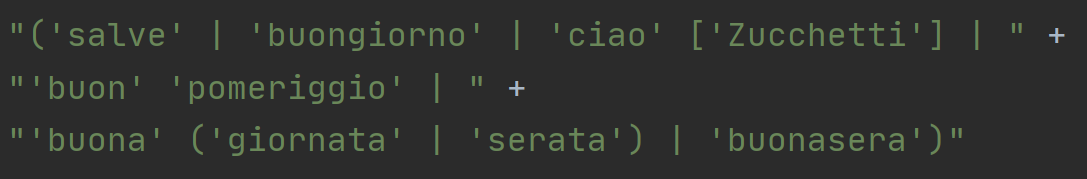
\includegraphics[height=1.7cm, width=\linewidth]{esempio-grammatica.PNG}
		\caption{Esempio di una grammatica}
	\end{center}
\end{figure}

\vspace{2cm}

Nonostante il loro principio di funzionamento sia relativamente semplice da comprendere, non sono altrettanto facili da interpretare se raggiungono grandi dimensioni, soprattutto per uno sviluppatore terzo che le dovrà riutilizzare in futuro. Per migliorare questo aspetto l'azienda ha deciso di utilizzare i diagrammi \emph{\gls{rldg}}\glsfirstoccur come strumento di rappresentazione come si può vedere nella figura successiva.

\begin{figure}[htbp]
	\begin{center}
		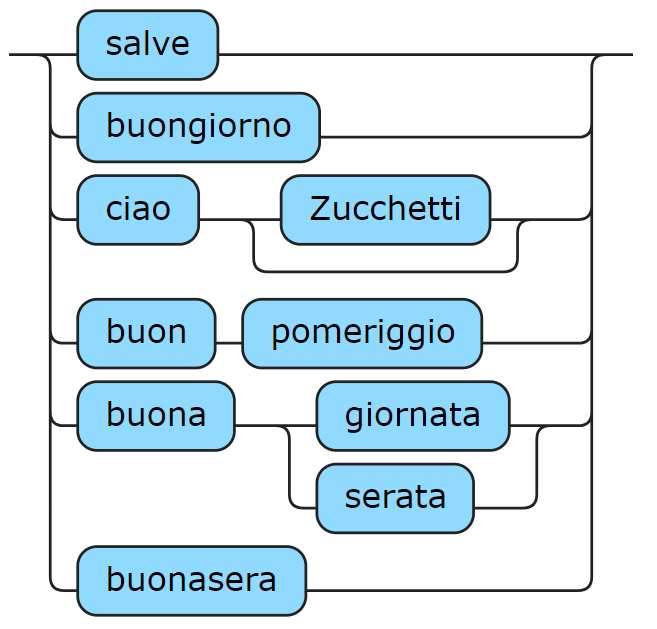
\includegraphics[height=6cm]{esempio-railroad.PNG}
		\caption{Esempio di una grammatica con railroad}
	\end{center}
\end{figure}

Risulta evidente infatti come questa raffigurazione sia molto più efficace e intuitiva. \\
Inoltre l'applicazione effettiva della \emph{\gls{gramg}} sugli input dell'utente avviene attraverso un apposito \emph{\gls{parsg}}\glsfirstoccur che mi è stato consegnato dall'azienda per lo sviluppo del progetto. \\
Infine per riassumere gli aspetti positivi e negativi di questa tecnologia viene presentato un paragone a quella attualmente utilizzata dagli assistenti virtuali presentati in precedenza. Non tutti i paragoni sono possibili a causa della mancanza di dati a disposizione ma viene comunque riportato nella seguente tabella.

\begin{table}
	\begin{tabularx}{\textwidth}{|X|X|X|}
		\hline
		\textbf{Caratteristica} & \textbf{Zucchetti} & \textbf{Aziende concorrenti} \\\hline
		
		Precisione nella comprensione & Estrema precisione: quando è compresa una frase si ha la certezza di averlo fatto correttamente.  & Buona precisione: quando è compresa una frase si ha buone probabilità di averlo fatto correttamente ma non la certezza. \\
		\hline
		Propensione alla comprensione & Comprende solo le frasi che lo sviluppatore mette a disposizione attraverso una \emph{\gls{gramg}}. & Cerca di interpretare anche frasi che non corrispondono esattamente a quelle a disposizione, talvolta commettendo degli errori. \\
		\hline
		Verbosità nello sviluppo & Poca verbosità in quanto, per costruzione, ad un aumento minimale vocaboli si ottiene un grande aumento delle frasi potenzialmente interpretabili. & Dati non disponibili. \\
		\hline
		Facilità della sintassi & Molto facili da gestire in quanto è basata su regole semplici che permettono di produrre molte frasi. & Dati non disponibili. \\
		\hline
		Prestazioni & Prestazioni molto elevate dovute ad un'ottima integrazione del \emph{\gls{parsg}} e all'esecuzione in locale, senza quindi onere nella comunicazione. & Prestazioni altrettanto elevate con l'incognita dei tempi di latenza dovuti all'esecuzione in remoto del \emph{\gls{parsg}} di interpretazione dell'input. \\
		\hline
	\end{tabularx}
	\caption{Tabella di confronto tra la tecnologia Zucchetti e quella dei concorrenti per l'interpretazione del linguaggio naturale}
\end{table}

\section{Analisi dei requisiti}
	\subsection{Descrizione del problema}
	Durante l'attività di ricerca sugli assistenti virtuali, in particolare nello sviluppo del \emph{\gls{pocg}} che fa uso di Alexa, è emerso un concetto importante, caratteristico anche del lavoro che sta svolgendo l'azienda: la conversazionalità. Essa rappresenta la capacità di intrattenere una conversazione da parte di un software simulando la presenza di una persona. \\
	Inoltre nella pianificazione del lavoro è inserita la costruzione di una \emph{\gls{nlug}} con relativa \emph{\gls{gramg}} che interpreti un insieme di frasi e dia una risposta ragionata sulla base di esse. \\
	È stato quindi deciso, in comune accordo con il tutor, di costruire un'applicazione che metta assieme la realizzazione di una propria \emph{\gls{nlug}} con capacità di conversazione finalizzata a soddisfare una determinata funzionalità e non limitata ad una coppia domanda-risposta. Il dominio dell'applicazione è simile a quello del \emph{\gls{pocg}} sviluppato con Alexa ovvero la data di nascita, solo che molto più completo. Le frasi pronunciabili dagli utenti per cui è prevista la comprensione sono  composte da:
	\begin{itemize}
		\item saluto iniziale opzionale;
		\item un insieme di frasi introduttive per esprimere la data di nascita nel formato giorno, mese e anno o, alternativamente, la data di compleanno nel formato giorno, mese;
		\item insieme di espressioni per la data di nascita e conseguentemente del sottoinsieme data di compleanno;
		\item insieme di frasi per riconoscere come data le espressioni che definiscono il giorno di Natale;
		\item insieme di frasi per riconoscere come data le espressioni che definiscono il primo giorno di un qualsiasi mese;
		\item insieme di frasi per interrompere l'esecuzione in qualunque momento;
		\item insieme di frasi per chiedere un eventuale aiuto sulle funzionalità offerte dell'applicazione.
	\end{itemize}
	\subsection{Requisiti}
	Lo scopo principale è dimostrare la fattibilità di implementare la capacità conversazionale in una \emph{\gls{nlug}} costruita con la tecnologia sviluppata da Zucchetti. L'applicazione perciò si presenta sotto forma di \emph{\gls{pocg}} e non è quindi integrata in un software aziendale esistente. \\
	Analizzando più in dettaglio gli obiettivi da raggiungere, è stata stilata una lista di requisiti obbligatori la cui fattibilità è certa. Uno tra quelli emersi, invece, è stato inserito come opzionale poiché rappresenta un miglioramento ragionevolmente non implementabile nel tempo a disposizione.
	I requisiti obbligatori sono i seguenti:
	\begin{enumerate}
		\item costruzione di una \emph{\gls{nlug}} che comprenda la data di nascita espressa dall'utente, esegua un'elaborazione e prepari una risposta adatta. Deve avere estrema precisione nella comprensione delle le frasi anche a costo di rigettarne alcune;
		\item implementazione della capacità conversazionale con relativa memoria che permetta di portare a compimento l'attività in esecuzione, provando a dare la percezione all'utente di dialogare con una persona. Più in dettaglio consiste nel richiedere i componenti mancanti della data di nascita o di compleanno oppure nella modifica dovuto a possibili errori, affinché l'utente li fornisca in modo completo e corretto;
		\item costruzione dell'interfaccia utente composta da:
		\begin{itemize}
			\item interfaccia grafica minimale che permetta all'utente di attivare il riconoscimento della voce;
			\item interfaccia vocale completa di tutti gli accessori studiati durante l'attività di ricerca. In input risulta essere una diretta conseguenza dello sviluppo della \emph{\gls{nlug}} mentre in output è progettata sulla base delle elaborazioni prodotte.
		\end{itemize}
	\end{enumerate}
	Il requisito opzionale è il seguente:
	\begin{enumerate}
		\item generalizzazione della grammatica che permetta non solo di interpretare l'input dell'utente ma anche di generare le risposta adeguate sulla base dell'elaborazione.
	\end{enumerate}
\section{Progettazione}
	\subsection{NLU}
	La \emph{\gls{nlug}} è il nucleo di tutto l'applicativo e la sua corretta progettazione è fondamentale. Essa consiste nella generazione di una \emph{\gls{gramg}} che interpreta l'input dell'utente e nella sua applicazione alle stringhe di testo. La \emph{\gls{gramg}} non è rappresentabile in un unico diagramma \emph{\gls{rldg}} in quanto ha dimensioni troppo elevate perciò sono illustrate le parti fondamentali. \\
	Il seguente diagramma rappresenta l'insieme di frasi per richiedere la data di nascita in cui prima viene detto il frammento di frase che corrisponde all'introduzione del contenuto come ad esempio "sono nato il" oppure "la mia data di nascita è" e successivamente il contenuto vero e proprio ovvero giorno, mese e anno in tutte le possibili combinazioni. 
		
	\begin{figure}[htbp]
		\begin{center}
			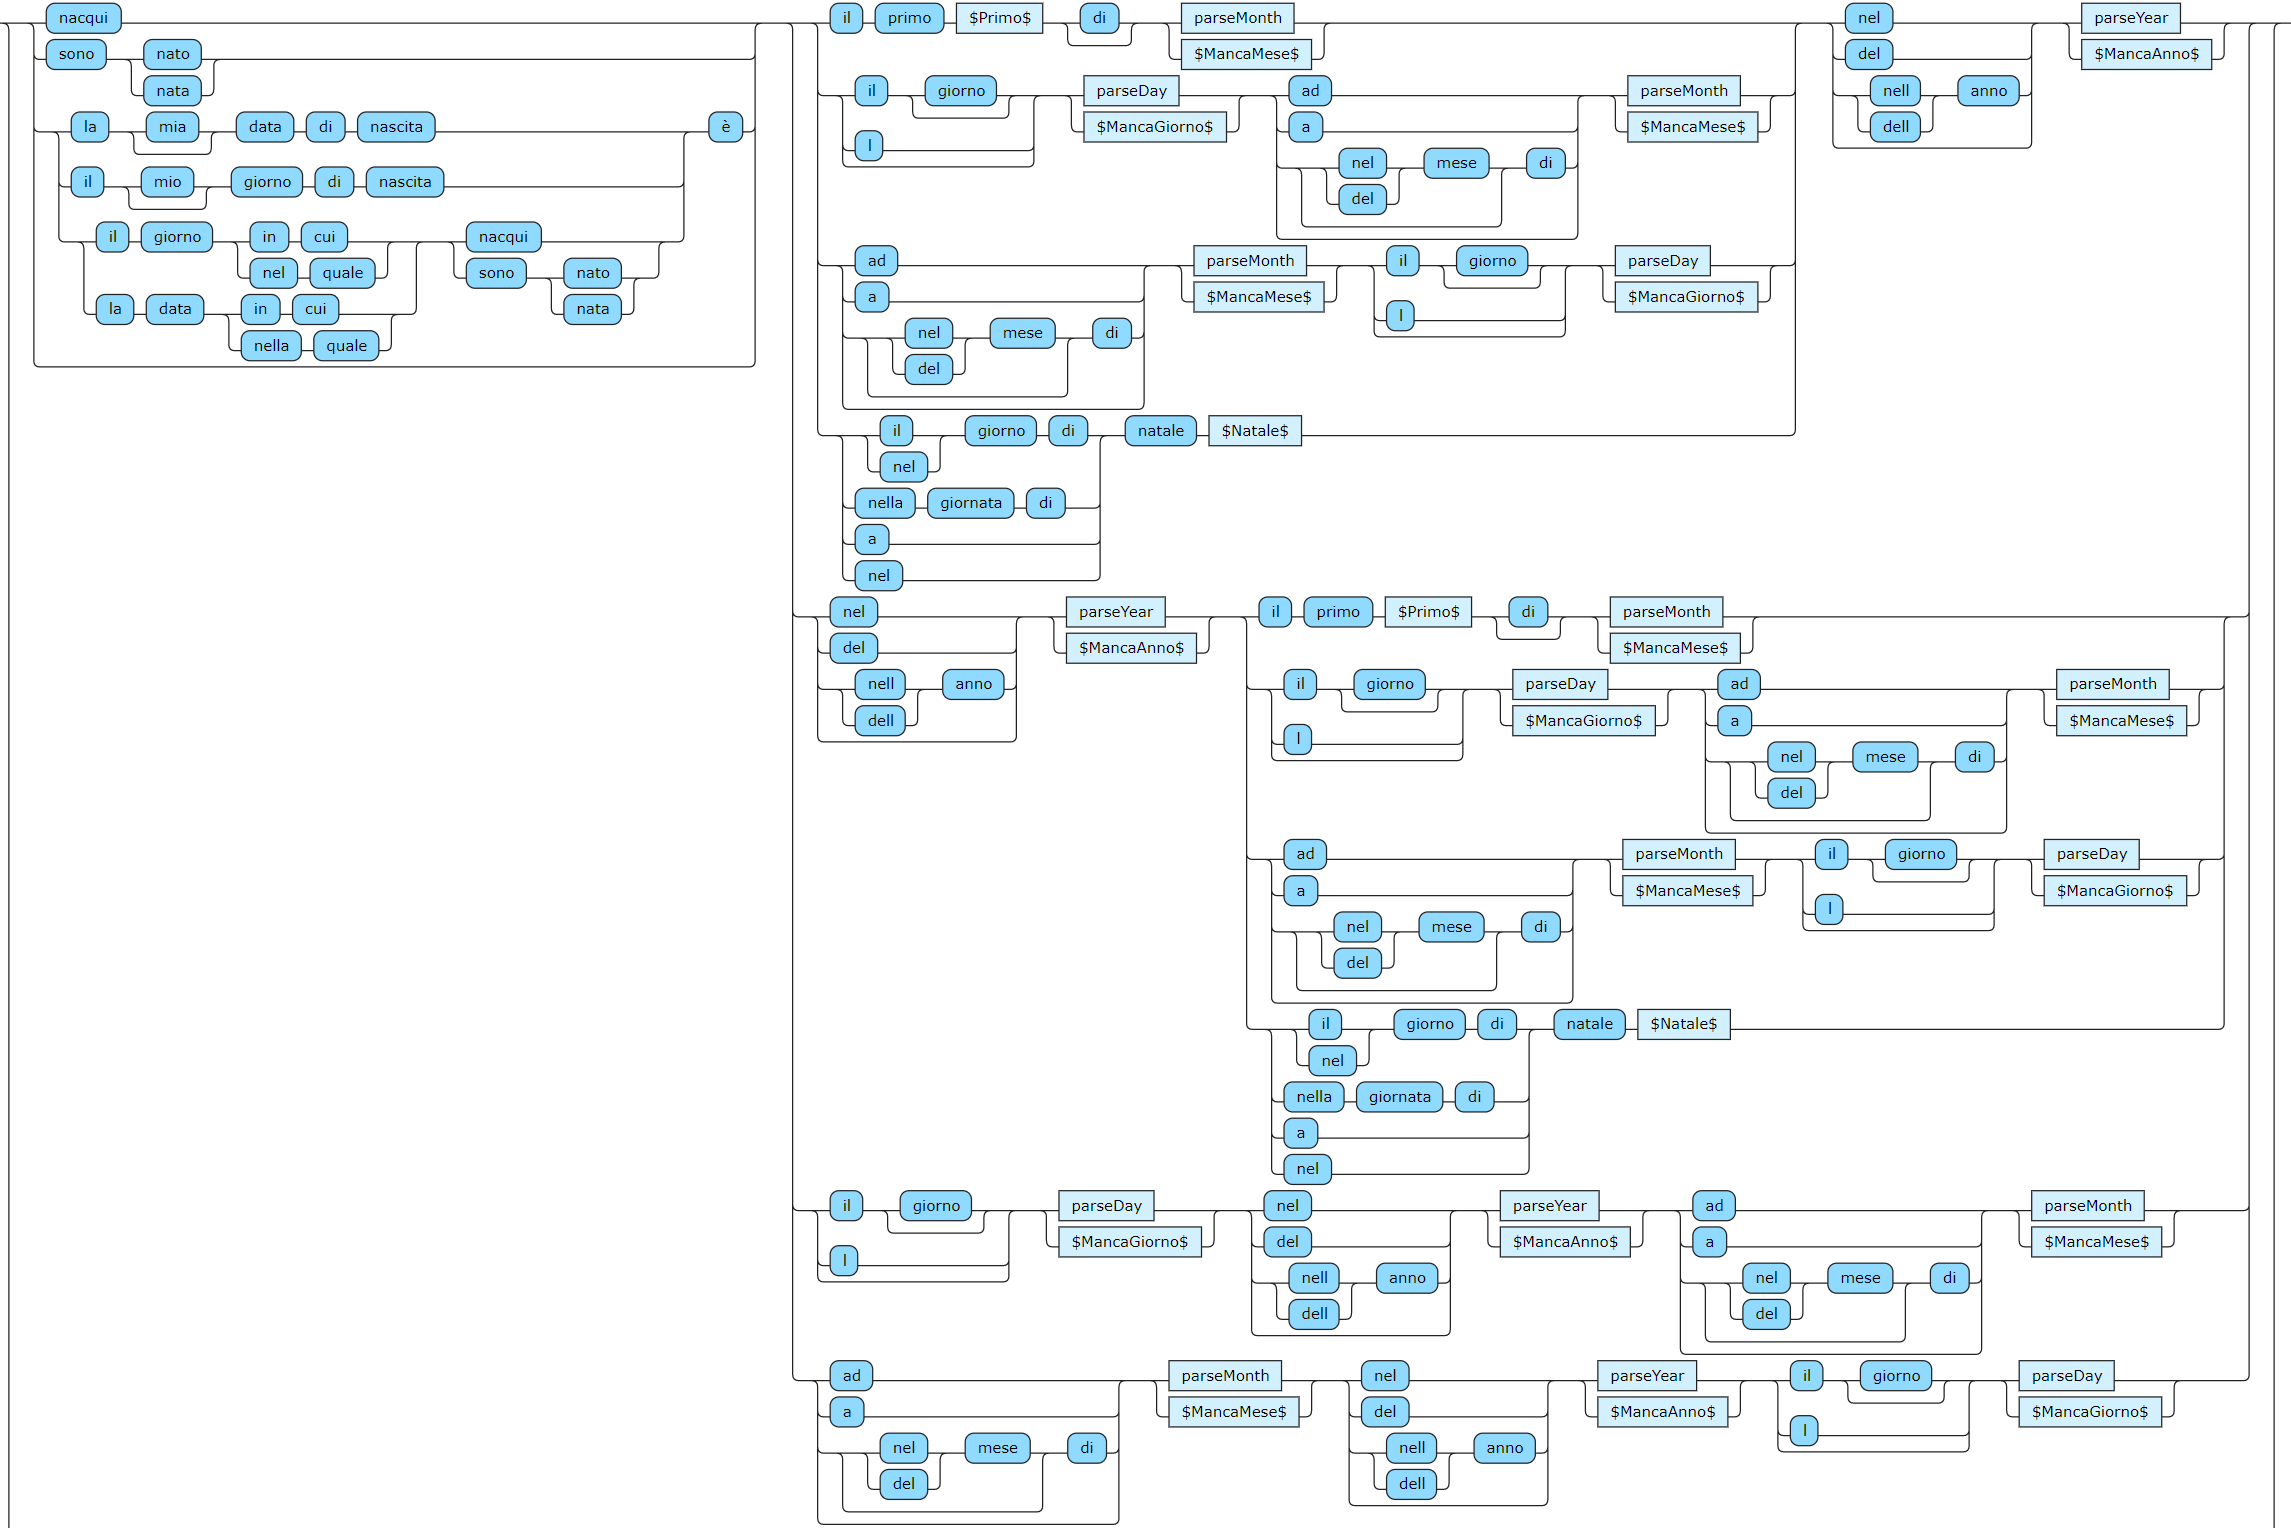
\includegraphics[height=10cm, width=\linewidth]{railroad_data_nascita.png}
			\caption{Diagramma railroad della grammatica per la data di nascita prima parte}
		\end{center}
	\end{figure}
	
	Nella figura successiva invece è rappresentato il diagramma \emph{\gls{rldg}} opposto in cui prima è previsto il contenuto ovvero giorno, mese e anno, sempre in tutte le possibili combinazioni, ed in seguito le sue frasi introduttive. Questo permette di riconoscere un maggior numero di versioni in cui l'utente può esprimere la data di nascita.
	
	\begin{figure}[htbp]
		\begin{center}
			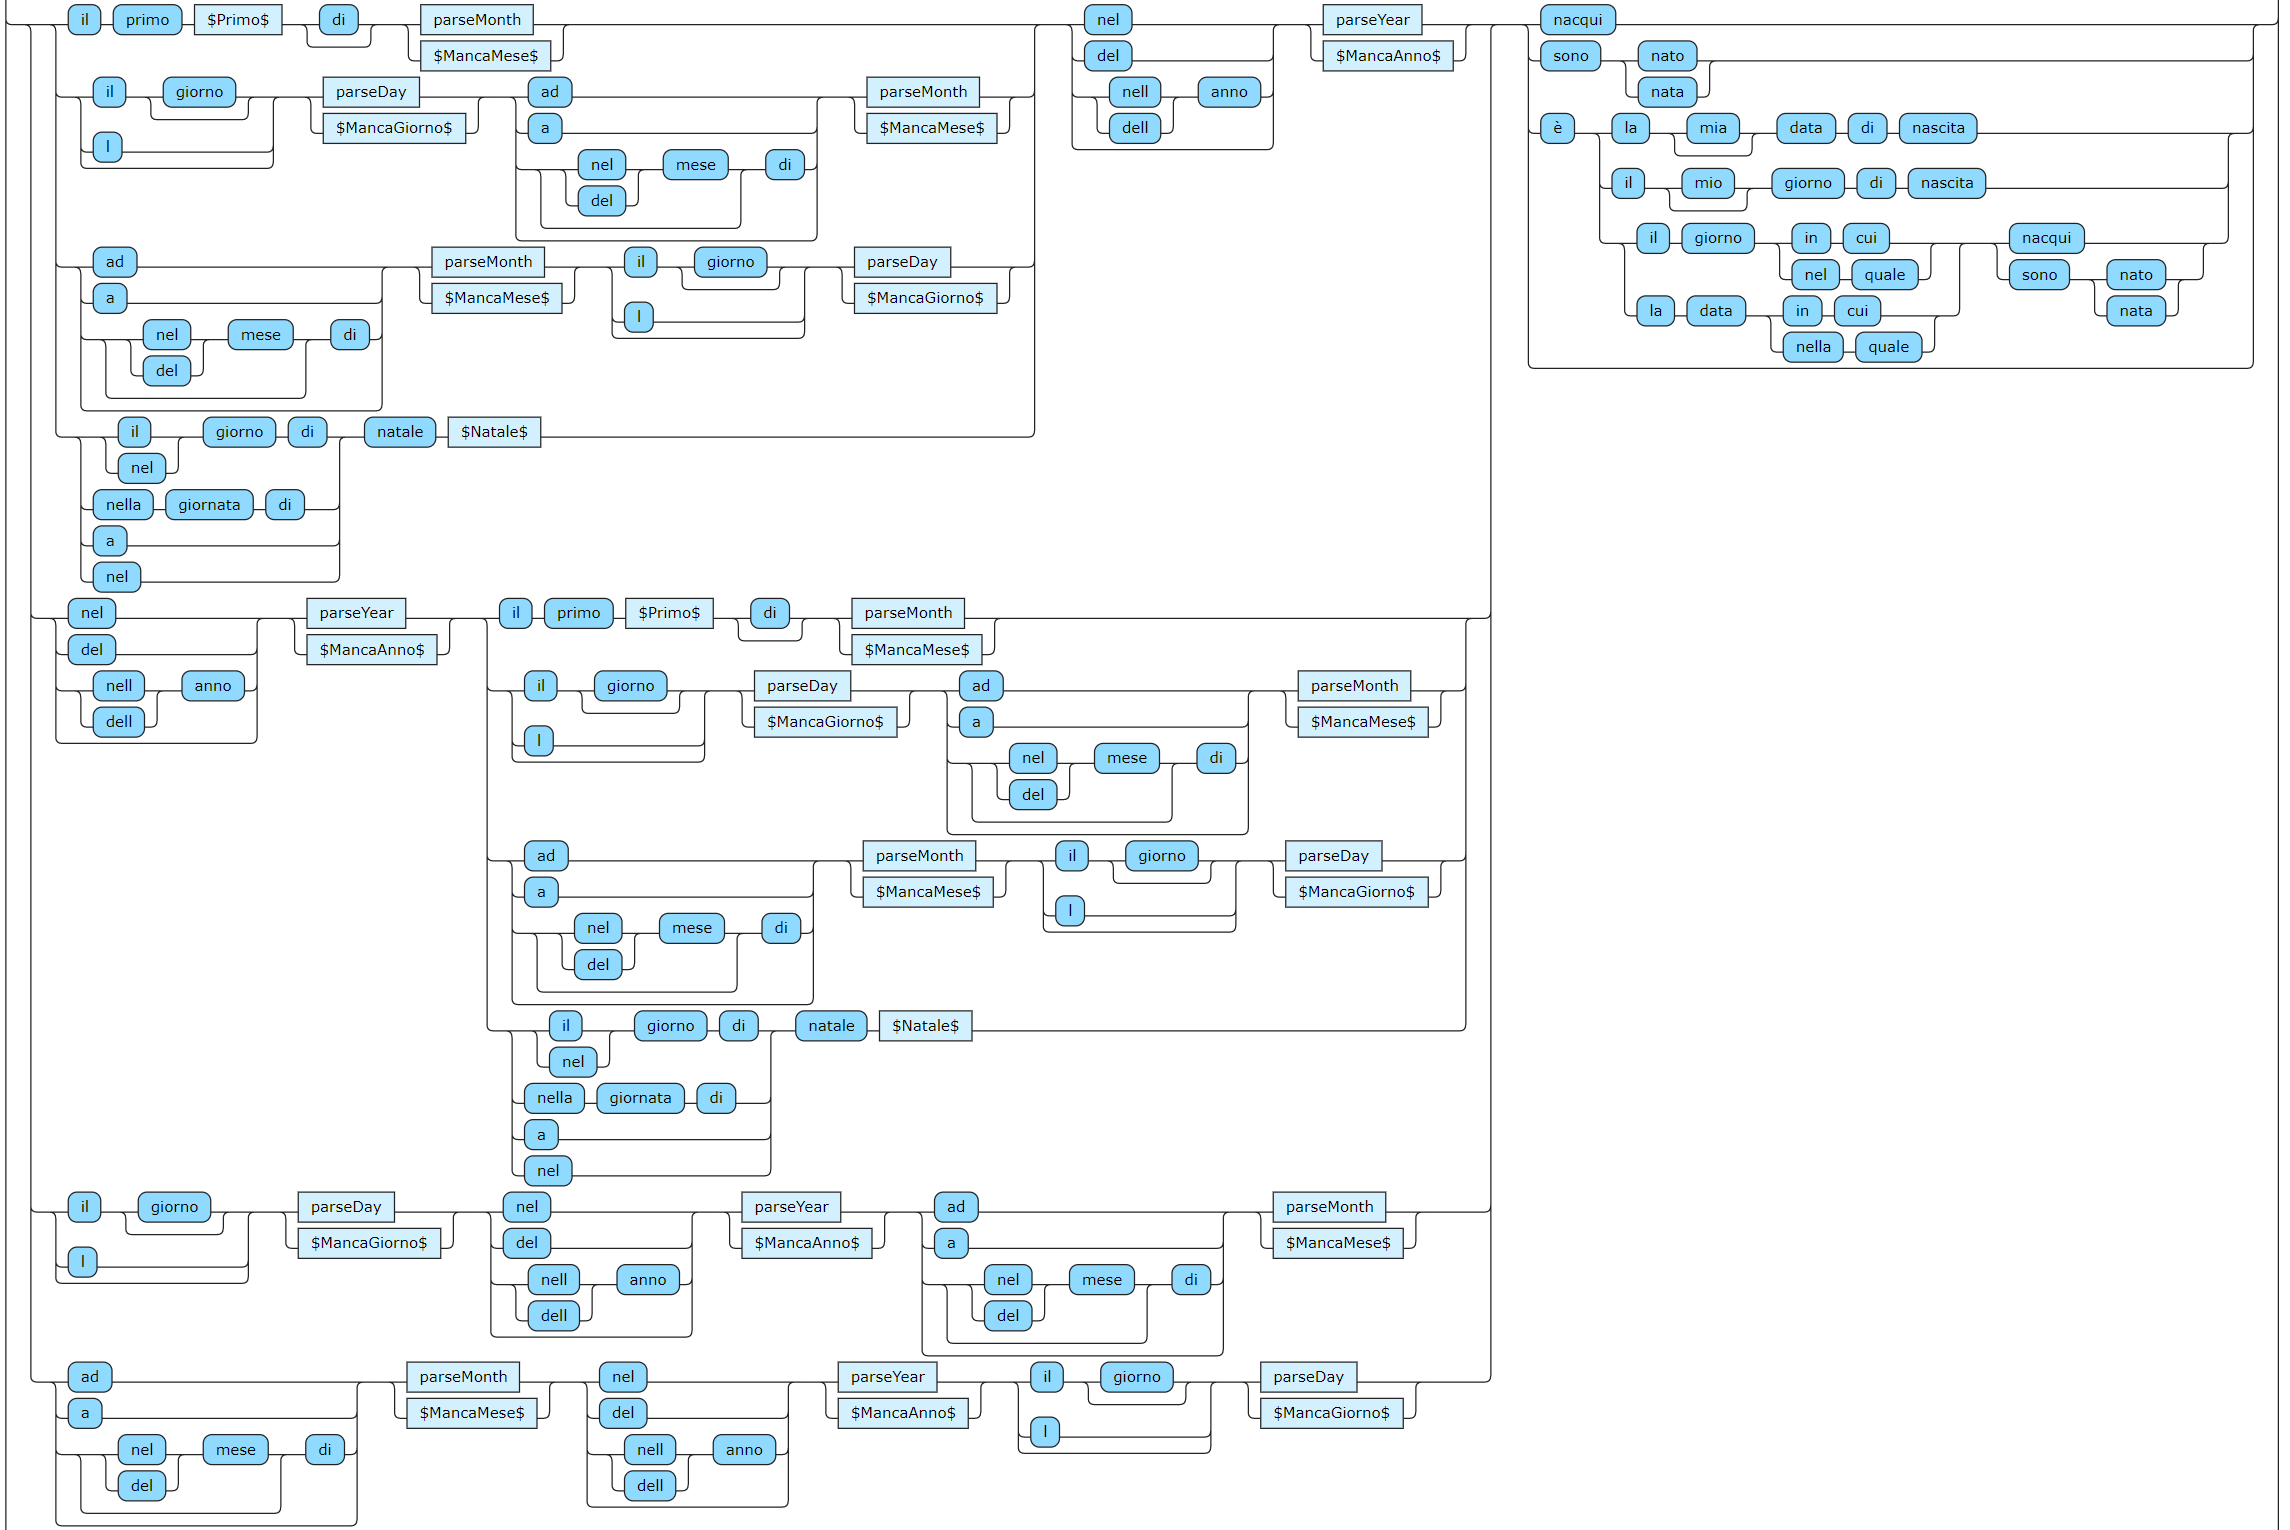
\includegraphics[height=10cm, width=\linewidth]{railroad_data_nascita_2.png}
			\caption{Diagramma railroad della grammatica per la data di nascita seconda parte}
		\end{center}
	\end{figure}

	Le due porzioni di \emph{\gls{gramg}} illustrate permettono globalmente di interpretare la data di nascita. Successivamente, seguendo lo stesso principio di separazione tra i frammenti di frase introduttivi e quelli di contesto, sono presentate le due porzioni di \emph{\gls{gramg}} che illustrano la data di compleanno, differente dalla precedente per l'assenza dell'anno. \\
	La figura seguente riporta la porzione che presenta prima la parte introduttiva e dopo quella di contenuto.
	
	\begin{figure}[htbp]
		\begin{center}
			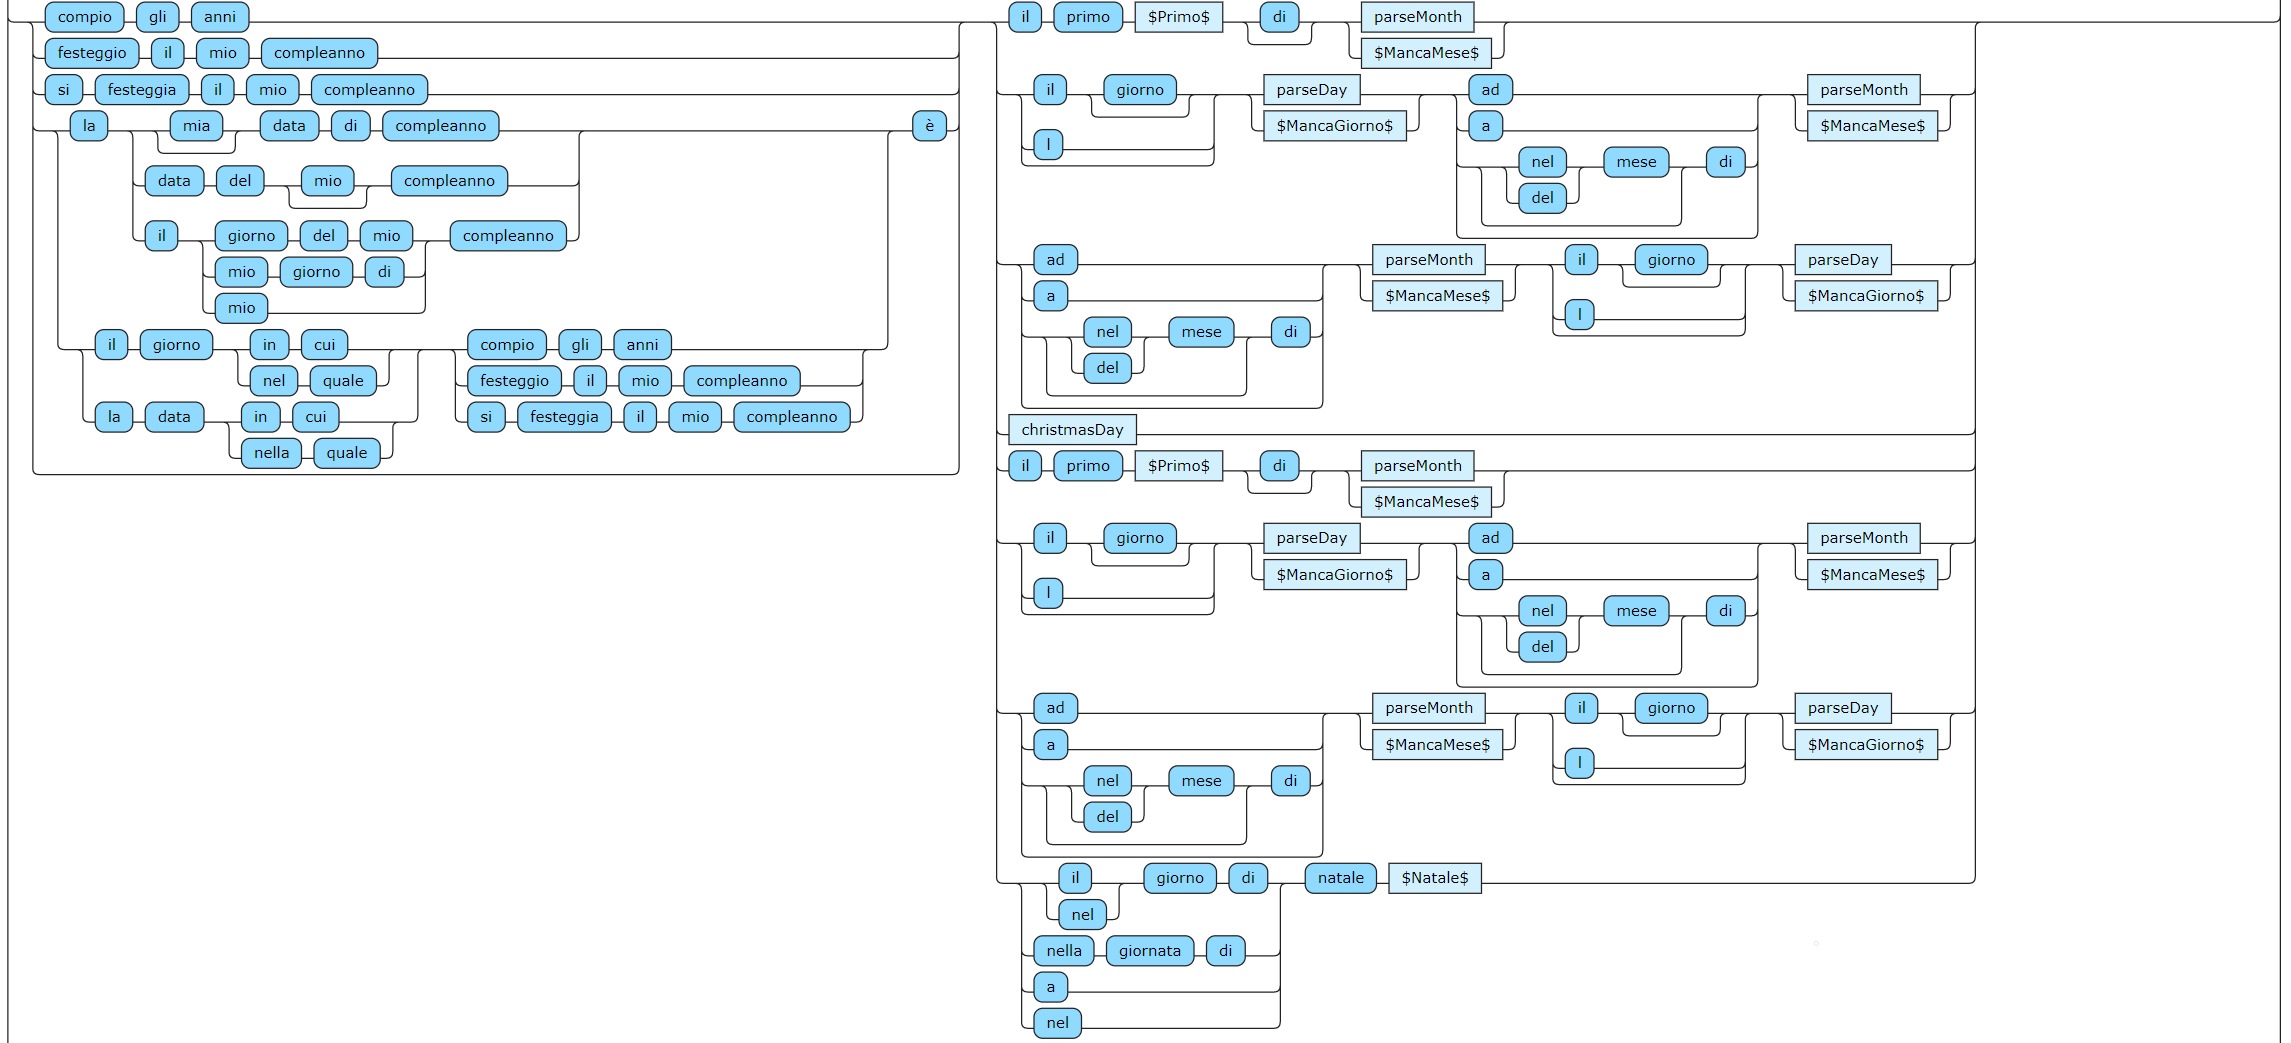
\includegraphics[height=8cm, width=\linewidth]{railroad_compleanno.png}
			\caption{Diagramma railroad della grammatica per il compleanno prima parte}
		\end{center}
	\end{figure}

	La prossima figura, invece, riporta la porzione che presenta prima la parte di contenuto e dopo quella introduttiva.
	\begin{figure}[htbp]
		\begin{center}
			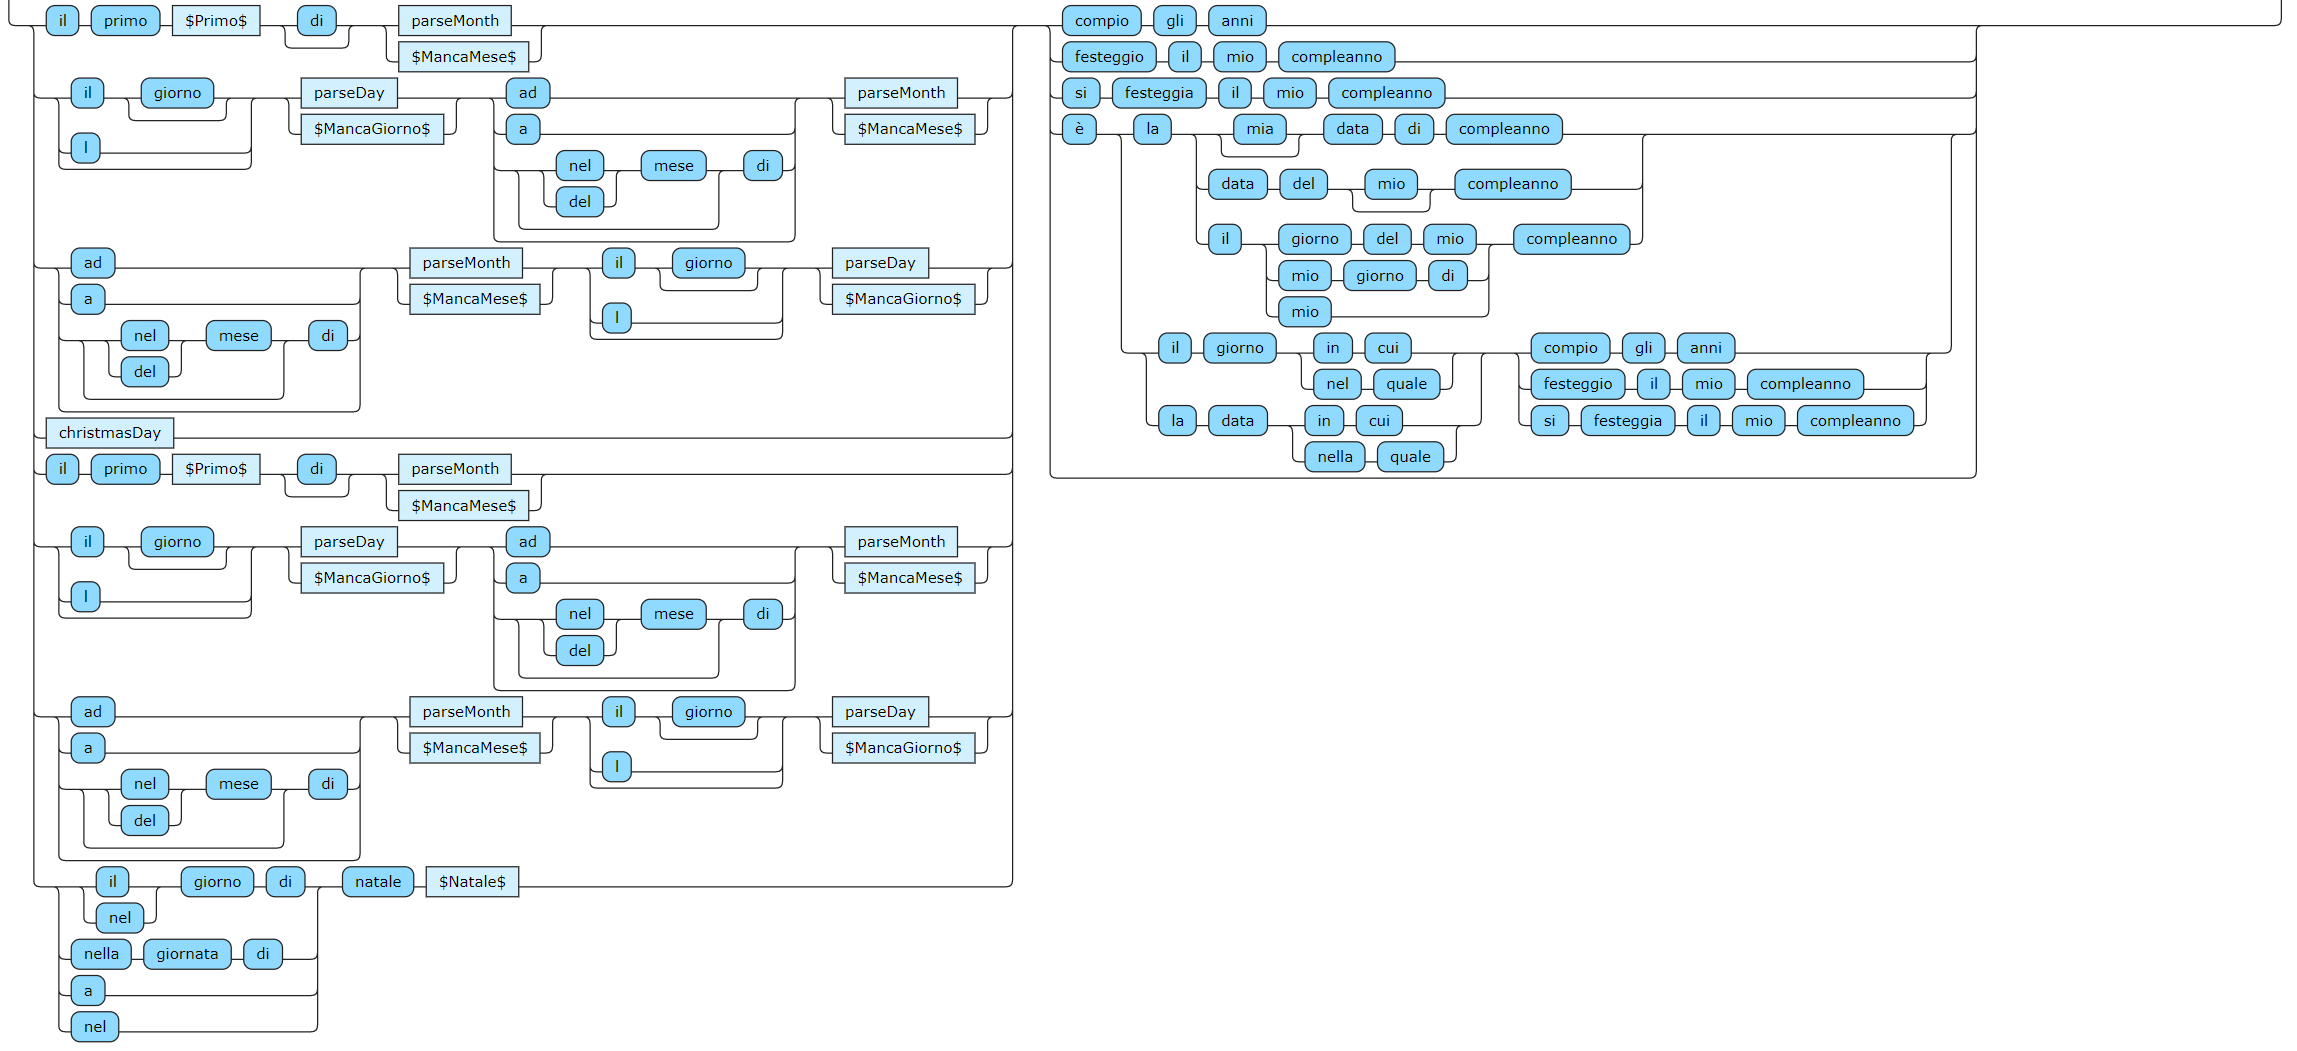
\includegraphics[height=8cm, width=\linewidth]{railroad_compleanno_2.png}
			\caption{Diagramma railroad della grammatica per il compleanno seconda parte}
		\end{center}
	\end{figure}

	\subsection{Capacità conversazionale}
	Nella progettazione della capacità conversazionale il concetto fondamentale è la memoria. Infatti, mentre la \emph{\gls{nlug}} permette l'interpretazione del linguaggio naturale, la capacità conversazionale consente di mantenere il contesto durante l'intero dialogo. \\
	Ho deciso di tenere traccia dei dati che lo costituiscono all'interno di un oggetto che sarà resettato ad ogni nuova conversazione. In questo modo è possibile costruire delle risposte basate sul contesto per porre domande mirate ad ottenere gli eventuali dati mancanti ovvero giorno, mese e anno. \\
	Infine la \emph{\gls{gramg}} descritta in precedenza è stata progettata anche per riconoscere singole parti di contenuto e di conseguenza viene riutilizzata anche per l'implementazione della conversazione. 
	\subsection{Interfaccia utente}
	La progettazione dell'interfaccia utente si articola in due parti:
	\begin{itemize}
		\item interfaccia grafica;
		\item interfaccia vocale.
	\end{itemize}
		\subsubsection{Interfaccia grafica}
		L'interfaccia grafica è stata progettata con un numero di elementi minimali all'interno ed è illustrata nella seguente immagine.
		\begin{figure}[htbp]
			\begin{center}
				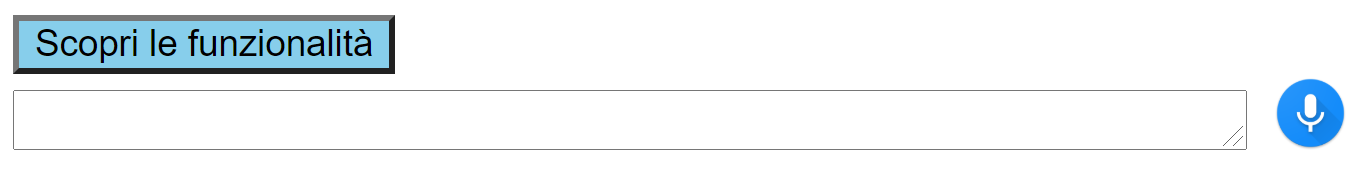
\includegraphics[height=1.7cm, width=\linewidth]{interfaccia-grafica.PNG}
				\caption{Interfaccia grafica dell'applicazione}
			\end{center}
		\end{figure}
	
		I componenti sono un pulsante che permette all'utente di ascoltare le funzionalità fornite, un pulsante con l'immagine del microfono che attiva il riconoscimento vocale ed una casella di testo non editabile che permetta di visualizzare il comando che è stato riconosciuto.		
		\subsubsection{Interfaccia vocale}
		L'interfaccia vocale è stata progettata con l'obiettivo di garantire la migliore esperienza possibile d'uso agli utenti. \\
		Ho utilizzato le nozioni apprese dalla documentazione degli assistenti virtuali analizzati per generare un'interfaccia vocale e sono:
		\begin{itemize}
			\item capire la tipologia degli utenti che deve interagire con la propria applicazione. In questo caso ha avuto importanza relativa in quanto si tratta di un \emph{\gls{pocg}} e non è stata prevista una categoria specifica;
			\item provare a costruire esempi di dialogo molteplici verificando quali risultano più naturali su un insieme di persone sia del team di sviluppo sia di altri impieghi. Nel mio caso l'ho provato con alcuni colleghi e persone esterne;
			\item scegliere uno stile di conversazione che si adatti maggiormente al contesto della propria applicazione;
			\item dare una spiegazione iniziale di ciò che si può dire o fare in caso di interfaccia grafica ausiliaria;
			\item valutare l'utilizzo di un'interfaccia grafica di ausilio per mantenere meglio il contesto, soprattutto se risulta corposo;
			\item gestire correttamente i possibili errori dovuti anche ad input scorretti dell'utente;
			\item dare la possibilità di chiedere aiuto l'utente in caso di difficoltà con frasi mirate;
			\item permette all'utente di interrompere l'esecuzione in qualsiasi momento senza dare la percezione di non poter uscire.
		\end{itemize}		
		Sulla base di queste indicazioni sono stati progettati tutti i componenti espressi nell'analisi. \\
		Per gli input dell'utente, l'interfaccia vocale è stata realizzata in conseguenza alla progettazione della \emph{\gls{gramg}}, per la quale sono comunque stati applicati i principi descritti mentre per l'output è stata personalizzata sulla base dell'elaborazione. Per la risposta si è infatti deciso di fornire un set di frasi con significato uguale ma con sintassi leggermente diversa, da cui viene scelta la frase a tempo di esecuzione secondo un algoritmo pseudo-casuale.
\section{Codifica}
Per realizzare l'interfaccia grafica ho implementato una semplice pagina in \emph{\gls{html}} con un altrettanto semplice foglio di stile in \emph{\gls{css}} per presentarla in modo più efficace. \\
Per realizzare i meccanismi di riconoscimento e di sintesi vocale ho utilizzato rispettivamente un componente jquery integrato in un'apposita classe Javascript che fornisce a tempo di esecuzione i diversi spezzoni di frase che sta riconoscendo e un oggetto della Web Speech \emph{\gls{apig}}. \\
Per utilizzare la \emph{\gls{nlug}} progettata ho realizzato una classe Javascript e simulato il meccanismo degli intenti %TODO:SISTEMA QUESTA PARTE
Per realizzare la capacità conversazionale ho creato due oggetti Javascript in cui il primo contiene giorno, mese, anno e contesto che può variare tra data di nascita e di compleanno mentre il secondo degli attributi booleani per giorno, mese e anno che se a true indicano un cambiamento rispetto a quanto espresso in precedenza. %TODO:Controlla che ci sia tutto

\section{Test}

\section{Sviluppi futuri}
Sarebbe stato possibile tenere traccia dei dati forniti dall'utente in modo permanente ad esempio all'interno di un database così che ad un nuovo utilizzo dell'utente l'applicazione si ricordasse di ciò che era stato detto precedentemente. Questo però pone alcuni vincoli quali un sistema di autenticazione dell'utente perciò diventa complesso.             % L'applicazione
% !TEX encoding = UTF-8
% !TEX TS-program = pdflatex
% !TEX root = ../tesi.tex

%**************************************************************
\chapter{Conclusione}
\label{cap:conclusione}
%**************************************************************

%\intro{Breve introduzione al capitolo}\\

%**************************************************************
\section{Consuntivo finale}
Gli scostamenti rilevati nelle prime tre attività sono dovuti alla difficoltà di reperimento di un computer con sistema operativo MacOS l'analisi e la costruzione del \emph{\gls{pocg}} relativo a Siri. Perciò si è deciso di privilegiare lo studio di Assistant ed Alexa con ulteriori approfondimenti. \\
Nelle attività finali, invece, si sono verificati degli scostamenti perché è stato svolto un approfondimento sulla possibile utilità del motore di regole a scapito, in comune accordo con il tutor aziendale, a scapito del tempo dedicato alla documentazione.
Il consuntivo finale è quindi riportato nella seguente tabella.
\begin{table}
	\begin{tabularx}{\textwidth}{|X|c|c|c|}
		\hline
		\textbf{Attività} & \textbf{Ore pianificate} & \textbf{Ore effettive} & \textbf{Scostamento} \\
		\hline
		Studio di Assistant e implementazione di un \emph{\gls{pocg}}. & 40 & 48 & +8 \\
		\hline
		Studio di Alexa e implementazione di un \emph{\gls{pocg}}. & 40 & 48 & +8 \\
		\hline
		Studio di Siri e implementazione di un \emph{\gls{pocg}}. & 40 & 32 & -8 \\
		\hline
		Test e documentazione comparativa di quanto svolto nelle settimane precedenti. & 40 & 40 & 0 \\
		\hline
		Apprendimento della tecnologia Zucchetti per il riconoscimento e l'elaborazione di comandi vocali. & 40 & 32 & -8 \\
		\hline
		Realizzazione di un'applicazione che implementi una \emph{\gls{nlug}} basata su una \emph{\gls{gramg}} costruita mediante la tecnologia di Zucchetti. & 40 & 40 & 0 \\
		\hline
		Implementazione della capacità conversazionale con scambio e memorizzazione di informazioni. & 40 & 48 & +8 \\
		\hline
		Test e documentazione di quanto svolto nelle settimane precedenti. & 40 & 32 & -8 \\	
		\hline
	\end{tabularx}
	\caption{Consuntivo finale}
\end{table}
\pagebreak
%**************************************************************
\section{Raggiungimento obiettivi}
Il raggiungimento degli obiettivi fa riferimento alla loro pianificazione descritta nella sezione §\hyperref[obiettivi]{2.2}.
\subsection{Obiettivi obbligatori}
\begin{itemize}
	\item \textbf{OB-1}: obiettivo raggiunto. Inizialmente è stata svolta un'analisi preliminare di tutte le capacità di Assistant e successivamente, sulla base di indicazioni e preferenze del tutor aziendale, sono state approfondite alcune singole funzionalità;
	\item \textbf{OB-2}: obiettivo raggiunto. Durante l'analisi delle capacità di Assistant è stato deciso di implementare un \emph{\gls{pocg}} legato alle App Actions;
	\item \textbf{OB-3}: obiettivo raggiunto. Inizialmente è stata svolta un'analisi preliminare di tutte le capacità di Alexa e successivamente, sulla base di indicazioni e preferenze del tutor aziendale, sono state approfondite alcune singole funzionalità;
	\item \textbf{OB-4}: obiettivo raggiunto. Durante l'analisi delle capacità di Alexa è stato deciso di implementare un \emph{\gls{pocg}} legato alle Skill con capacità conversazionale;
	\item \textbf{OB-5}: obiettivo raggiunto. È stato redatto un documento che riporta un'analisi dettagliata e comparativa degli assistenti virtuali studiati;
	\item \textbf{OB-6}: obiettivo raggiunto. Sono state studiate regole e caratteristiche della tecnologia Zucchetti per costruire \emph{grammatiche} che riconoscono il linguaggio naturale;
	\item \textbf{OB-7}: obiettivo raggiunto. In comune accordo con il tutor aziendale è stata realizzata un'applicazione con una propria \emph{\gls{nlug}} basata su una \emph{\gls{gramg}} generata tramite la tecnologia Zucchetti. Il suo scopo principale è riconoscere ed elaborare la data di nascita e di compleanno dell'utente interagendo mediante un'interfaccia vocale.
\end{itemize}
\subsection{Obiettivi desiderabili}
\begin{itemize}
	\item \textbf{OD-1}: obiettivo raggiunto. Implementazione della capacità conversazionale mirata a reperire e memorizzare tutti i dati relativi a data di nascita e di compleanno dell'utente per soddisfare lo scopo dell'applicazione.
\end{itemize}
\subsection{Obiettivi facoltativi}
\begin{itemize}
	\item \textbf{OF-1}: obiettivo raggiunto. Inizialmente è stata fatta un'analisi preliminare di tutte le capacità di Siri e successivamente, sulla base di indicazioni e preferenze del tutor aziendale, sono state approfondite le singole funzionalità;
	\item \textbf{OF-2}: obiettivo non raggiunto. Durante l'analisi delle capacità di Siri è stato deciso di implementare un \emph{\gls{pocg}} che permetta l'utilizzo delle Shortcuts. Tuttavia a causa delle restrizioni dell'account sviluppatore Apple a disposizione non si è potuta portare a compimento tale attività.
\end{itemize}
\subsection{Tabella riassuntiva}
\begin{table}
	\begin{tabularx}{\textwidth}{|c|X|c|}
		\hline
		\textbf{Codice} & \textbf{Obiettivo} & \textbf{Esito} \\
		\hline
		OB-1 & Studio e analisi delle capacità e delle modalità di utilizzo lato sviluppatore di Assistant. & Raggiunto \\
		\hline
		OB-2 & Implementazione di un \emph{\gls{pocg}} che realizzi una funzionalità di Assistant accordata sulla base dei risultati della ricerca. & Raggiunto \\
		\hline
		OB-3 & Studio e analisi delle capacità e delle modalità di utilizzo lato sviluppatore di Alexa. & Raggiunto \\
		\hline
		OB-4 & Implementazione di un \emph{\gls{pocg}} che realizzi una funzionalità di Alexa accordata sulla base dei risultati della ricerca. & Raggiunto \\
		\hline
		OB-5 & Redazione di un documento che riporta un'analisi dettagliata e comparativa degli assistenti virtuali studiati. & Raggiunto \\
		\hline
		OB-6 & Studio di regole e caratteristiche dell'algoritmo di Zucchetti per la costruzione di \emph{grammatiche} che riconoscono il linguaggio naturale. & Raggiunto \\
		\hline
		OB-7 & Realizzazione di un'applicazione con una propria \emph{\gls{nlug}} basata su una \emph{\gls{gramg}} generata mediante la tecnologia Zucchetti che interagisca con gli utenti tramite interfaccia vocale. & Raggiunto \\
		\hline
		OD-1 & Implementazione della capacità conversazionale tramite lo scambio di informazioni specifiche, possibilmente memorizzate, durante la conversazione mirato a soddisfare una determinata funzionalità. & Raggiunto \\	
		\hline
		OF-1 & Studio e analisi delle capacità e delle modalità di utilizzo lato sviluppatore di Siri. & Raggiunto \\	
		\hline
		OF-2 & Implementazione di un \emph{\gls{pocg}} che realizzi una funzionalità di Siri accordata sulla base dei risultati della ricerca. & Non raggiunto\\	
		\hline
	\end{tabularx}
	\caption{Raggiuntimento degli obiettivi}
\end{table}
\pagebreak
%**************************************************************
\section{Valutazione personale}
\subsection{Conoscenze acquisite}
Durante l'attività di stage ho acquisto numerose conoscenze affrontando argomenti non presenti nel mio piano di studi universitario e ampliate altre che avevo appreso negli anni precedenti. Esse sono riportate nel seguente elenco:
\begin{itemize}
	\item principi e funzionalità degli assistenti virtuali: ho scoperto molte funzionalità degli assistenti virtuali che ho riportato nel capitolo  §\hyperref[cap:descrizione-stage]{3} ma soprattutto ho appreso molte nozioni sul loro funzionamento e su come possono essere utili sia agli utenti nella loro vita quotidiana sia alle azienda nella realizzazione dei loro prodotti. Le due principali sono il meccanismo degli intenti che rappresenta un nuovo modo di gestire l'interazione con gli utenti e l'insieme dei principi di realizzazione dell'interfaccia vocale che rappresentano un nuovo modo di interagire con gli utenti ancora poco esplorato ma ricco di potenzialità. Questi sono stati inoltre sperimentati nell'applicazione costruita;
	\item costruzione di applicazioni Android: durante lo sviluppo del \emph{\gls{pocg}} relativo ad Assistant ho imparato da autodidatta le basi della costruzione di un'applicazione Android con il linguaggio Kotlin e come attivarne le funzionalità tramite Assistant;
	\item costruzione di applicazioni in linguaggio Swift per l'ecosistema Apple: durante lo sviluppo del \emph{\gls{pocg}} relativo a Siri ho imparato da autodidatta le basi della costruzione di un'applicazione per iOS in linguaggio Swift e come predisporre delle Shortcuts personalizzabili dall'utente e attivabili tramite Siri;
	\item utilizzo di Javascript in ambiti nuovi: lo sviluppo dell'applicazione, a parte l'interfaccia grafica, è interamente realizzato in Javascript. Ho quindi imparato a realizzare software scritti in questo linguaggio per scopi diversi da quelli presentati durante il mio percorso di studi ed inoltre questo mi ha fatto capire la grande versatilità e l'ampio utilizzo che ne viene fatto nella costruzione di applicazioni;
	\item comprensione del linguaggio naturale: la tecnologia Zucchetti per l'interpretazione del linguaggio naturale si basa sull'utilizzo di \emph{grammatiche} per le quali ho avuto una formazione teorica durante il mio percorso di studi ma grazie a questa esperienza ho imparato ad implementarle. Ho inoltre appreso i principi di realizzazione di una \emph{\gls{nlug}}, oltre a metodologie per l'elaborazione dei risultati, e delle numerose problematiche e difficoltà che ne derivano;
	\item capacità di utilizzare nuovi strumenti: la varietà di tecnologie affrontate mi ha portato ad imparare l'utilizzo di altrettanti strumenti ausiliari quali Xcode, AndroidStudio e i diagrammi \emph{\gls{rldg}}.
\end{itemize}
\subsection{Competenze acquisite}
Grazie all'esperienza di stage, oltre alle conoscenze, ho acquisito nuove competenze che mi hanno permesso di maturale molto a livello professionale. Esse sono riportate nel seguente elenco:
\begin{itemize}
	\item versatilità nell'utilizzo e nell'apprendimento di nuove tecnologie: la maggior parte dello stage è stato centrata su analisi e apprendimento di molte tecnologie, talvolta diverse tra loro. Ciò mi ha permesso di migliorare nell'approccio alla ricerca, nell'autoapprendimento e nella capacità di fare paragoni definendo vantaggi e svantaggi;
	\item capacità di elaborare ragionamenti in ottica di innovazione: uno degli scopi principali delle mie ricerche è stato capire quali delle funzionalità e degli strumenti offerti fossero utili ai progetti aziendali. Esse infatti sono state riportate e discusse più volte con il mio tutor ed altri colleghi in sede di \emph{\gls{brainstorming}}\glsfirstoccur. Questo mi ha permesso contribuire ed imparare a fare dei ragionamenti mirati all'innovazione e al miglioramento a prodotti già esistenti o in via di sviluppo.
\end{itemize}
\subsection{Tecnologie e strumenti utilizzati}
Le tecnologie e gli strumenti con cui ho lavorato sono numerosi. Nella realizzazione dei \emph{\gls{pocg}} legati agli assistenti virtuali ho utilizzato Kotlin con Android Studio nell'applicazione per Assistant, Javascript con la console da sviluppatori nella Skill per Alexa e Swift con Xcode nell'applicazione per Siri. \\
Per l'applicazione che implementa la \emph{\gls{nlug}}, invece, ho utilizzato HTML e CSS per l'interfaccia grafica e Javascript versione \emph{\gls{es6}} per tutte le altre componenti mentre come strumento ho utilizzato WebStorm. \\
La maggior parte di queste tecnologie non sono state affrontate, oppure solo in modo marginale, durante il mio percorso di studi; tuttavia quella di cui ho avvertito maggior carenza è indubbiamente Javascript in quanto ne ho fatto largo uso in ambiti totalmente nuovi.
\subsection{Metodologia di lavoro}
Lo stage si è svolto in remoto e questa è stata una nuova esperienza sia per me che per il mio tutor. Per cercare di simulare nel modo migliore possibile la presenza in azienda siamo rimasti in contatto quotidianamente e, in aggiunta, ho redatto un registro riportando ogni giorno tutte le attività svolte. \\
Lo svantaggio riscontrato dal lavoro in remoto è la mancanza del rapporto diretto con il tutor ed i colleghi che, a mio parere, è formativo dal punto vista sia personale che professionale. Tuttavia porta con sé alcuni vantaggi quali maggior flessibilità negli orari e la non necessità di viaggiare in auto per recarsi in ufficio. Inoltre, soprattutto per lavori in ambito informatico, esistono numerosi strumenti che permettono di lavorare da casa in modo efficace ed efficiente annullando parte degli svantaggi. \\
Perciò è stata una sfida ed una possibilità di sperimentare una nuova modalità di lavoro che mi ha permesso ugualmente di raggiungere gli obiettivi prefissati con risultati notevoli.
\subsection{Analisi retrospettiva dei risultati}
Il lavoro svolto durante lo stage non è stato strutturato per realizzare un prodotto finito e pronto all'uso ma per eseguire una ricerca esplorativa su argomenti di interesse per i progetti aziendali, che trova concretezza in alcuni \emph{\gls{pocg}} dimostrativi. In seguito ho analizzato i risultati ottenuti e da essi sono emersi degli ottimi spunti di riflessione. \\
Il primo è: dall'interfaccia vocale l'utente si aspetta intelligenza. Questo l'ho percepito durante lo sviluppo dell'applicazione, quando ancora non c'era una copertura sufficiente nella comprensione dei comandi vocali. Infatti, mentre facevo eseguire dei test ad alcuni utenti esterni, spesso la \emph{\gls{nlug}} non riusciva a comprendere le frasi pronunciate facendoli spazientire; loro si aspettavano di colloquiare con un sistema intelligente al pari di una persona. Inoltre, se si considera l'aspetto conversazionale, il problema diventa ancora più accentuato in quanto l'utente si aspetta di interagire con un software che comprenda il contesto del dialogo in corso e abbia capacità di memoria. \\
Questa considerazione ha grande rilevanza perché evidenzia l'attenzione ai minimi dettagli che si deve prestare durante la progettazione dell'interfaccia vocale. Infatti, nonostante i grandi vantaggi che porta, quali la velocità e la comodità di utilizzo, presenta dei rischi notevoli sulla sua buona riuscita nei confronti degli utenti. \\
La seconda riflessione, invece, è la seguente: l'utilizzo dell'interfaccia vocale deve essere giustificato rispetto a quella grafica. Questa considerazione nasce dal fatto che l'interfaccia grafica è in assoluto la più diffusa, grazie anche ai dispositivi mobili, diventando lo standard per gli utenti. Il vantaggio dell'interfaccia vocale però risiede nella maggior comodità e rapidità legata all'esecuzione di operazioni semplici per le quali quindi risulta giustificata; tuttavia in attività complesse, possibilmente svolte in ambienti rumorosi, risulta assai svantaggiosa e lo sforzo per implementarla può non essere pienamente giustificato. \\
L'utilizzo di un'interfaccia vocale con una \emph{\gls{nlug}} rappresenta senza dubbio una tecnologia con grandi potenzialità ancora inesplorate ma dalle due precedenti riflessioni emergono i suoi limiti attuali. \\
La terza riflessione si propone come una possibile idea per risolvere i problemi riscontrati: costruire un'interfaccia ibrida che metta assieme gli aspetti positivi di quella vocale e di quella grafica. Più nello specifico mi riferisco alla costruzione di un'interfaccia che da un lato abbia una componente grafica per gli elementi più complessi e rilevanti in modo che l'utente non percepisca senso di smarrimento o difficoltà nell'utilizzo e dall'altro abbia una componente vocale per le operazioni più facili e di immediata esecuzione. In questo modo si eviterebbero buona parte dei problemi espressi in precedenza senza però sfruttarne a pieno le potenzialità. \\
La quarta ed ultima riflessione si stacca leggermente dalle precedenti poiché si sofferma sull'interfaccia vocale e sul possibile pattern architetturale di applicazioni che ne fanno uso. Questa riflessione è emersa in uno degli ultimi colloqui con il tutor aziendale in riferimento al pattern Model-View-Controller ed è la seguente: la View è per natura una componente passiva che esegue il rendering del modello e non possiede stato; tuttavia questo diventa impossibile da applicare con l'interfaccia vocale e la motivazione risiede nella capacità conversazionale che si vuole offrire all'utente. Più in dettaglio la View contiene sempre tutto quello che l'utente deve vedere mentre durante una conversazione il contesto si costruisce nel tempo rendendo impossibile presentare l'intero contenuto. Inoltre questo contesto, che necessariamente deve essere memorizzato, non appartiene propriamente al modello dell'applicazione in quanto non rappresenta nè i dati nè le operazioni da eseguire e nemmeno al Controller perché ha mansioni totalmente differenti. Perciò tali considerazioni portano a pensare che sia legati alla View. Da qui nasce l'idea che il pattern Model-View-Controller non sia direttamente applicabile a programmi basati su interfaccia vocale ma necessiti di una modifica nella View, trasformandola in un componente con capacità di memoria che mantiene il contesto della conversazione. \\
Queste sono le riflessioni esprimono l'esito conclusivo dell'analisi retrospettiva dei risultati riscontrati durante lo stage. \\
Infine io sono rimasto molto soddisfatto dagli argomenti trattati, dalla tipologia di lavoro svolto, dal rapporto lavorativo con il tutor aziendale ed in generale dall'intera esperienza.

%TODO: Impatto del lavoro sul progetto aziendale generale (il prodotto è utilizzato?), possibili punti di insoddisfazione e relativi miglioramenti ed estensioni
%TODO: VEDI FOGLIO RIASSUNTIVO ULTIMI RAGIONAMENTI SVOLTI
%todo: COMMENTI PERSONALI FINALI

             % Conclusioni
%% !TEX encoding = UTF-8
% !TEX TS-program = pdflatex
% !TEX root = ../tesi.tex

%**************************************************************
\chapter{Conclusioni}
\label{cap:conclusioni}
%**************************************************************

%**************************************************************
\section{Consuntivo finale}

%**************************************************************
\section{Raggiungimento degli obiettivi}

%**************************************************************
\section{Conoscenze acquisite}

%**************************************************************
\section{Valutazione personale}
%**************************************************************            % Conclusioni
%\input{capitoli/capitolo-7}            % Conclusioni
%\appendix                               
%\input{capitoli/capitolo-A}             % Appendice A


%**************************************************************
% Materiale finale
%**************************************************************
\backmatter
\printglossary[type=acronym, title={Acronimi e abbreviazioni}]
\printglossary[type=main, title={Glossario}]
% !TEX encoding = UTF-8
% !TEX TS-program = pdflatex
% !TEX root = ../tesi.tex

%**************************************************************
% Bibliografia
%**************************************************************

\cleardoublepage
\chapter{Bibliografia}
TODO
%\nocite{*}
% Stampa i riferimenti bibliografici
%\printbibliography[heading=subbibliography,title={Riferimenti bibliografici},type=book]

% Stampa i siti web consultati
%\printbibliography[heading=subbibliography,title={Siti web consultati},type=online]


\end{document}
